% =============================================================
%  MAIN FILE — MD Engine Project Report
%  Course: Electronic Structure & Atomistic Modeling of Materials
%
%  COLLABORATION INSTRUCTIONS:
%  Each section lives in its own file inside /sections/.
%  Assign one file per person. Edit only your own file.
%  Only touch main.tex to add/reorder \input{} lines.
% =============================================================

\documentclass[12pt, a4paper]{article}

% ---------- Packages ----------
\usepackage[top=2.5cm, bottom=2.5cm, left=3cm, right=3cm]{geometry}
\usepackage{amsmath, amssymb}
\usepackage{graphicx}
\usepackage{float}
\usepackage{booktabs}
\usepackage{hyperref}
\usepackage{xcolor}
\usepackage{listings}
\usepackage{caption}
\usepackage{subcaption}
\usepackage{fancyhdr}
\usepackage{titlesec}
\usepackage{parskip}
\usepackage{setspace}
\usepackage{enumitem}
\usepackage{multirow}
\usepackage{array}
\usepackage{tikz}
\usepackage{pgfplots}
\pgfplotsset{compat=1.18}

% ---------- Hyperref setup ----------
\hypersetup{
    colorlinks=true,
    linkcolor=blue!60!black,
    citecolor=green!50!black,
    urlcolor=blue,
}

% ---------- Code listing style ----------
\lstdefinestyle{python}{
    language=Python,
    basicstyle=\ttfamily\small,
    keywordstyle=\color{blue}\bfseries,
    commentstyle=\color{gray}\itshape,
    stringstyle=\color{orange!80!black},
    numberstyle=\tiny\color{gray},
    numbers=left,
    stepnumber=1,
    numbersep=8pt,
    backgroundcolor=\color{gray!8},
    frame=single,
    rulecolor=\color{gray!40},
    breaklines=true,
    showstringspaces=false,
    tabsize=4,
    captionpos=b,
}
\lstset{style=python}

% ---------- Section title formatting ----------
\titleformat{\section}{\large\bfseries\sffamily}{}{0em}{\thesection\quad}
\titleformat{\subsection}{\normalsize\bfseries\sffamily}{}{0em}{\thesubsection\quad}
\titleformat{\subsubsection}{\normalsize\itshape\sffamily}{}{0em}{\thesubsubsection\quad}

% ---------- Header / Footer ----------
\pagestyle{fancy}
\fancyhf{}
\rhead{\small MD Simulation — Krypton}
\lhead{\small ESAM Project Report}
\rfoot{\small\thepage}
\renewcommand{\headrulewidth}{0.4pt}

% ---------- Custom commands ----------
\newcommand{\rstar}{r^{*}}
\newcommand{\tstar}{t^{*}}
\newcommand{\Tstar}{T^{*}}
\newcommand{\Estar}{E^{*}}
\newcommand{\rhostar}{\rho^{*}}
\newcommand{\gr}{g(r)}
\newcommand{\eps}{\varepsilon}

% =============================================================
\begin{document}

% ---------- Title Page ----------
\begin{titlepage}
    \centering
    \vspace*{2cm}

    {\Large\sffamily\bfseries Electronic Structure \& Atomistic Modeling of Materials}\\[0.5em]
    {\large\sffamily Course Project}

    \vspace{1.5cm}
    \rule{\linewidth}{1.5pt}\\[0.4em]
    {\Huge\bfseries\sffamily Build Your Own\\[0.3em] MD Simulation}\\[0.4em]
    \rule{\linewidth}{1.5pt}

    \vspace{1.5cm}
    {\large\itshape Molecular Dynamics Engine for Krypton}\\[0.3em]
    {\normalsize Property Studied: Radial Distribution Function $g(r)$}

    \vspace{2cm}
    \begin{tabular}{rl}
        \textbf{Group Members:} & Devadath Sabarish \\
                                & Guddeti Sreeteja \\
                                & Himesh Katru \\
                                & Tanish Verma \\[1em]
        \textbf{Roll Numbers:}  & CO24BTECH11006 \\
        & CO24BTECH11009 \\
        & CO24BTECH11010 \\
        & CO24BTECH11023 \\[1em]
        \textbf{Submitted to:}  & Anuj Goyal \\[1em]
        \textbf{Date:}          & \today \\
    \end{tabular}

    \vfill
    {\small Department of Computational Engineering\\[0.2em]
    Indian Institute of Technology Hyderabad}
\end{titlepage}

% ---------- Abstract ----------
% =============================================================
%  SECTION: Abstract
%  ASSIGNED TO: [Person Name]
% =============================================================

\newpage
\begin{abstract}
\noindent
% Write a concise summary (150–200 words) covering:
%  - What was built (MD engine, 6 modules)
%  - What was simulated (Krypton, LJ potential, FCC lattice)
%  - What was observed (solid→liquid transition via g(r))
%  - Key quantitative result (e.g., melting occurs near T* ≈ ?)
%
% [WRITE ABSTRACT HERE]

\end{abstract}


% ---------- Table of Contents ----------
\newpage
\tableofcontents
\newpage

% =============================================================
%  PART I: MODULE-WISE IMPLEMENTATION AND TESTING
% =============================================================
\part*{Module-wise Implementation and Testing}
\addcontentsline{toc}{part}{Module-wise Implementation and Testing}

% =============================================================
%  SECTION: Module 1 — The Physics of Interaction
% =============================================================

\newpage
\section{Module 1: The Physics of Interaction}

\subsection{What Are We Doing?}

At its heart, an MD simulation is a machine that answers one question repeatedly: \textit{given where all the atoms are right now, what force does each one feel?} Before we can integrate Newton's equations or build a simulation box, we need a mathematical rule that tells us how strongly two atoms push or pull each other at any distance. Module 1 implements that rule — the \textbf{Lennard-Jones (LJ) potential} — and extracts from it both the potential energy and the interatomic force for every pair of atoms in the system.

\subsection{Why Are We Doing It?}

\subsubsection{Why the Lennard-Jones Potential?}

Think about what happens as two inert gas atoms are brought progressively closer together from infinity. Far apart, they barely notice each other — the interaction is negligible. As they approach, the fluctuating electron clouds on each atom begin to induce temporary dipoles in the other, creating a weak but real attractive pull. This is the \textbf{van der Waals (dispersion) force}, and quantum mechanics tells us it decays precisely as $1/r^6$.

Keep pushing the atoms closer and something changes dramatically. Below a certain distance, the electron clouds begin to overlap. The Pauli exclusion principle prevents two electrons from occupying the same quantum state, so the energy shoots up steeply — this is \textbf{Pauli repulsion}. While the true quantum-mechanical form is exponential, Lennard-Jones approximated it with a $1/r^{12}$ power law, chosen cleverly because $r^{12} = (r^6)^2$: the repulsive term costs only one extra multiplication to compute from the attractive term.

The result is a simple two-parameter model that captures the full story of inert-gas interactions:
\begin{equation}
    \phi(r_{ij}) = 4\epsilon \left[\left(\frac{\sigma}{r_{ij}}\right)^{12} - \left(\frac{\sigma}{r_{ij}}\right)^{6}\right]
    \label{eq:lj_real}
\end{equation}
where $\sigma$ is the distance at which the potential crosses zero (the effective atomic diameter), and $\eps$ is the depth of the energy well (the strength of the interaction). For Krypton: $\sigma_\text{Kr} = 3.65$\,\AA\ and $\eps_\text{Kr}/k_B = 162.46$\,K.

\subsubsection{Why Use Reduced Units?}

Writing a simulation in SI units is a recipe for numerical disaster. The mass of a Krypton atom is $1.39 \times 10^{-25}$\,kg, a typical distance is $3.65 \times 10^{-10}$\,m, and a typical energy is $2.24 \times 10^{-21}$\,J. Storing, multiplying, and comparing numbers with such vastly different exponents introduces floating-point rounding errors that accumulate over thousands of timesteps.

The fix is to measure everything in the system's \emph{own} natural units, built from $\sigma$, $\eps$, and the atomic mass $m$:
\begin{equation}
    r^* = \frac{r}{\sigma}, \quad
    \phi^* = \frac{\phi}{\eps}, \quad
    t^* = \frac{t}{\sigma\sqrt{m/\eps}}
    \label{eq:reduced_units}
\end{equation}
In these reduced units, the LJ potential becomes elegantly parameter-free:
\begin{equation}
    \phi^*(\rstar) = 4\left[\frac{1}{(\rstar)^{12}} - \frac{1}{(\rstar)^{6}}\right]
    \label{eq:lj_reduced}
\end{equation}
Every quantity is now of order 1, numerical errors are minimised, and — crucially — the same simulation code represents \emph{any} inert gas species. Switching from Argon to Krypton simply means rescaling the output, not rewriting the code.

\subsubsection{Why Shift the Potential at the Cutoff?}

Computing the LJ interaction between every pair of atoms is an $O(N^2)$ bottleneck. We break this by introducing a \textbf{cutoff radius} $r_c^* = 2.5$: pairs further apart than $r_c^*$ contribute zero force and are ignored entirely. The potential at the cutoff is small but not exactly zero: $\phi^*(r_c^*) \approx -0.0163$.

Without a correction, an atom crossing the cutoff boundary would experience an instantaneous \emph{jump} in energy — the system suddenly gains or loses $\phi^*(r_c^*)$ for free. Over thousands of timesteps, these jumps accumulate and the total energy drifts, violating conservation and invalidating the simulation. The fix is the \textbf{shifted potential}: simply subtract $\phi^*(r_c^*)$ from the potential everywhere, so the curve smoothly reaches zero at the cutoff with no discontinuity:
\begin{equation}
    \phi^*_\text{shift}(\rstar) = \phi^*(\rstar) - \phi^*(r_c^*)
    \label{eq:lj_shifted}
\end{equation}

\subsection{How Is It Implemented?}

\subsubsection{Computing Energy and Force from $r^2$}

The function \texttt{calculate\_lj\_properties} takes as input $r^2$ (not $r$) and returns \newline$(\phi^*_\text{shift},\; F^*/r^*)$. Working in $r^2$ throughout is a standard MD optimisation: computing $r$ from $r^2$ requires an expensive square root, but the LJ formula only ever needs even powers of $r$. All inverses are built from $1/r^2$:
\begin{equation}
    \frac{1}{r^{*6}} = \left(\frac{1}{r^{*2}}\right)^3, \qquad
    \frac{1}{r^{*12}} = \left(\frac{1}{r^{*6}}\right)^2
\end{equation}
saving two expensive operations per pair.

\subsubsection{Why Return $F^*/r^*$, Not $F^*$?}

The scalar LJ force magnitude is obtained from the potential gradient:
\begin{equation}
    F^* = -\frac{d\phi^*}{dr^*} = \frac{48}{r^{*13}} - \frac{24}{r^{*7}}
        = \frac{48}{r^{*2}}\left(\frac{1}{r^{*12}} - \frac{1}{2\,r^{*6}}\right) \cdot r^*
    \label{eq:force}
\end{equation}
To get the 3D force \emph{vector} on atom $i$ from atom $j$, we need to multiply by the unit vector $\hat{\mathbf{r}}_{ij} = \mathbf{r}_{ij}/r$. Combining:
\begin{equation}
    \mathbf{F}^*_i = \frac{F^*}{r^*} \cdot \mathbf{r}_{ij}
    \label{eq:force_vector}
\end{equation}
By returning $F^*/r^*$ directly, the function avoids computing $r^*$ at all — the displacement vector $\mathbf{r}_{ij}$ is already available from the distance calculation, and the scalar $F^*/r^*$ can be applied to it directly.

\subsubsection{The Full Potential Curve}

Figure~\ref{fig:lj_curves} shows both the unshifted and shifted potential (left panel) and the force $F^*/r^*$ (right panel). The four key features to notice are:
\begin{enumerate}
    \item $\phi^*(r^*=1) = 0$ — the potential crosses zero at $r^* = \sigma^* = 1$, the atomic diameter.
    \item The minimum $\phi^* = -1$ occurs at $r^*_\text{min} = 2^{1/6} \approx 1.122$ — the equilibrium bond length.
    \item The shifted curve smoothly touches zero at $r_c^* = 2.5$ with no jump.
    \item $F^*/r^*$ is positive (repulsive) for $r^* < 2^{1/6}$ and negative (attractive) for $r^* > 2^{1/6}$, reaching zero at the equilibrium distance.
\end{enumerate}

\begin{figure}[H]
    \centering
    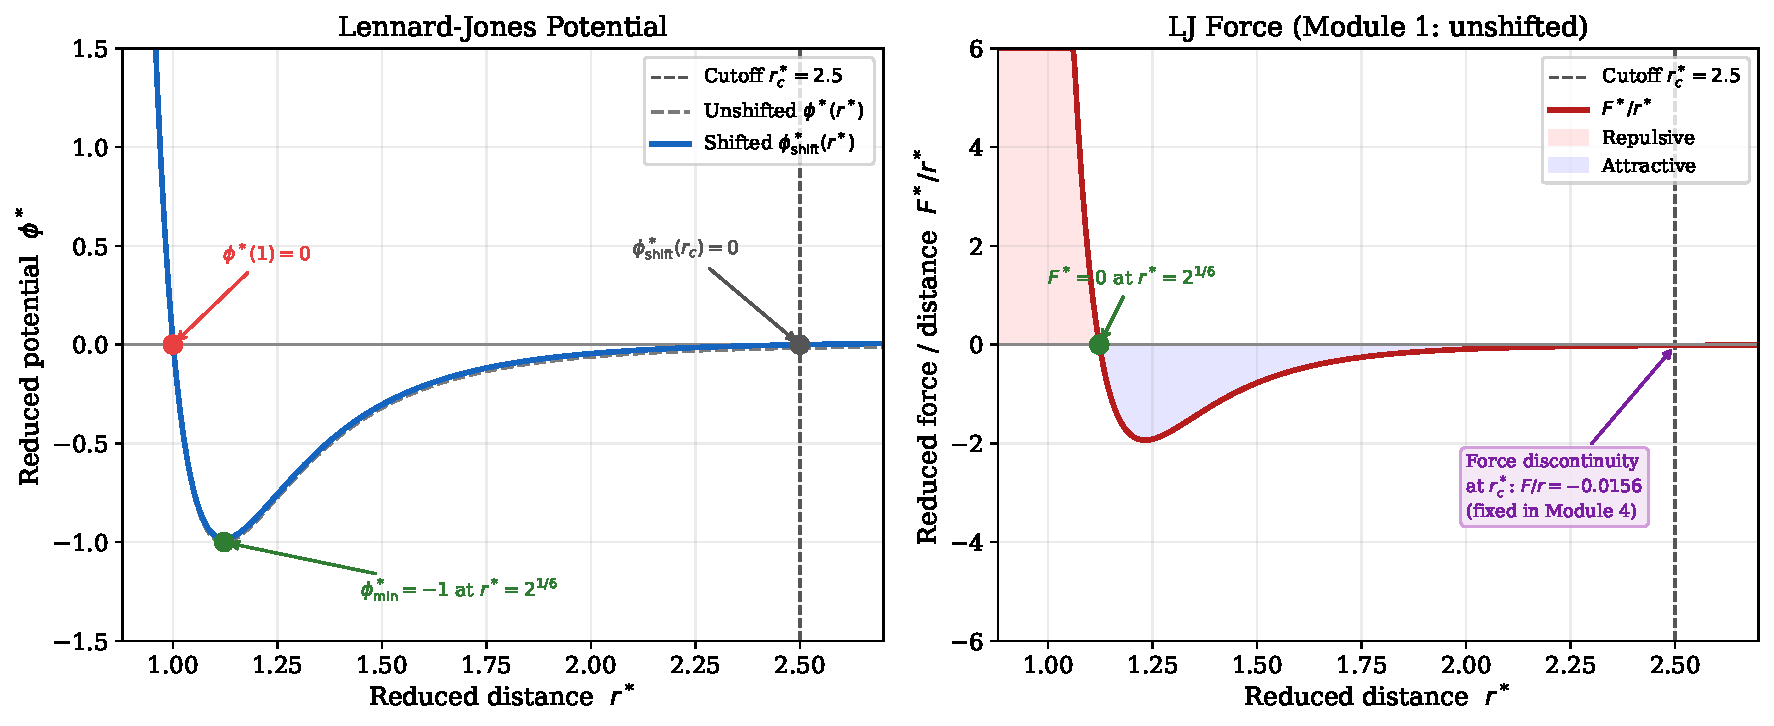
\includegraphics[width=\linewidth]{figures/m1_lj_curves.pdf}
    \caption{Lennard-Jones potential and force in reduced units for cutoff $r_c^* = 2.5$. \textbf{Left:} The unshifted $\phi^*(r^*)$ (dashed) and the shifted potential $\phi^*_\text{shift}$ (solid blue) as implemented in Module 1. The shift moves the curve down so it hits exactly zero at the cutoff, eliminating the energy discontinuity. \textbf{Right:} The force divided by distance, $F^*/r^*$. The shaded regions highlight the repulsive ($r^* < 2^{1/6}$) and attractive ($r^* > 2^{1/6}$) regimes. The labelled discontinuity at $r_c^*$ in the force — not present in the potential — is resolved in Module 4.}
    \label{fig:lj_curves}
\end{figure}

\subsection{Test Results}

Three unit tests were run on \texttt{calculate\_lj\_properties} to verify correctness before integration into the MD engine.

\begin{table}[H]
    \centering
    \caption{Module 1 verification tests with $r_c^* = 2.5$.}
    \label{tab:m1_tests}
    \begin{tabular}{llccc}
        \toprule
        \textbf{Test} & \textbf{Input $r^*$} & \textbf{Quantity checked} & \textbf{Expected} & \textbf{Obtained} \\
        \midrule
        1. Zero-point    & $1.0$         & Unshifted $\phi^*(1)$         & $0.000000$   & $0.000000$ \\
                         &               & Force/r sign                  & $> 0$ (repulsive) & $+24.0$ \\[4pt]
        2. Minimum energy & $2^{1/6} \approx 1.1225$ & Unshifted $\phi^*_\text{min}$ & $-1.000000$ & $-1.000000$ \\
                         &               & Force/r at minimum            & $\approx 0$  & $-2.1\times10^{-15}$ \\[4pt]
        3. Cutoff shift  & $r_c^* = 2.5$ & Shifted $\phi^*(r_c^*)$       & $0.000000$   & $0.000000$ \\
                         &               & Force/r at $r_c^*$            & non-zero     & $-0.0156$ \\
        \bottomrule
    \end{tabular}
\end{table}

All three tests pass exactly. A few observations are worth noting. In Test 1, the \emph{shifted} potential at $r^*=1$ is $+0.0163$, not zero — the shift raises the whole curve by $|\phi^*(r_c^*)| = 0.0163$, so the zero-crossing moves slightly to the right of $r^* = 1$. This is expected and physically harmless. In Test 2, the force at the energy minimum is $-2.1\times10^{-15}$ — effectively zero to machine precision, confirming the function correctly identifies the equilibrium distance. In Test 3, the shifted potential is exactly zero at the cutoff (no energy jump), but the force is $-0.0156$: Module 1 shifts \emph{only} the energy, not the force. This small but non-zero force discontinuity is addressed in Module 4 with the shifted-force potential.

% =============================================================
%  SECTION: Module 2: Boundary Conditions and Geometry
% =============================================================

\newpage
\section{Module 2: Boundary Conditions and Geometry}

\subsection{What Are We Doing?}

Before we can run any simulations, we must address three straightforward questions:

\textbf{1. Where should we place the atoms?} In a real bulk material, atoms are surrounded by neighbors in all directions. Our simulation, however, can only contain a few hundred atoms, forcing us to choose where to position them. Randomly placing atoms seems simplest but is catastrophic: overlaps are nearly inevitable, and the simulation interprets overlapping electron clouds as violent collisions, accelerating atoms violently in the first time step and crashing the program.

\textbf{2. How do we handle the finite boundaries of our simulation box?} A real material extends indefinitely, with atoms deep in the interior fully surrounded by neighbors. Our simulation cell, by contrast, has hard walls. Atoms near these boundaries lack neighbors on one side and therefore behave unphysically, exhibiting altered thermal and structural properties. We need a way to eliminate artificial surface effects and simulate bulk behavior.

\textbf{3. How do we correctly compute interactions in a periodic system without infinite calculations?} Periodic Boundary Conditions create an infinite array of replicated cells to mimic bulk material. This raises a new problem: without careful treatment, an atom would need to interact with infinitely many copies of every other atom, making the simulation computationally impossible.

Module 2 presents three techniques that resolve all three issues: the Minimum Image Convention (MIC), Periodic Boundary Conditions (PBC), and the Face-Centred Cubic (FCC) lattice.

\subsection{Why Are We Doing It?}

\subsubsection{Why the FCC Lattice and Not Random Positions?}

The reduced Lennard-Jones potential (Eq.~\eqref{eq:lj_reduced}) has a $1/(r^*)^{12}$ repulsive core that grows \emph{extremely} steeply as two atoms approach each other. If we place atoms at random positions, there is a high probability that some pair will overlap, say $r^* \approx 0.5$, where the potential energy soars to $\phi^* \approx 4[(1/0.5)^{12} - (1/0.5)^6] \approx 16000$. In the NVE ensemble\footnote{The NVE ensemble represents an isolated system where the Number of particles, Volume, and total Energy remain strictly constant throughout its lifetime.}, total energy is conserved, so this enormous potential energy converts instantly into kinetic energy. The atoms fly apart at absurd speeds, and the simulation diverges.

Starting on an FCC lattice avoids this entirely. Inert gas solids like Krypton naturally crystallize into the FCC structure, so along with the initial condition being computationally safe, it is also physically motivated. Every atom begins with well-separated, regular neighbours, and the system can equilibrate smoothly toward thermodynamic equilibrium.

\subsubsection{Why Periodic Boundary Conditions and Not Just a Box with Walls?}

In a real material containing on the order of $10^{23}$ atoms, those deep in the interior are fully surrounded by neighbours, while only a very small fraction reside at the surface. In contrast, in a simulation with just $N = 256$ atoms confined in a simple box with hard walls, nearly half of the atoms lie close to a wall and therefore lack neighbours on one side. This leads to a serious issue. Atoms at the surface act very differently from those in the bulk, because they're missing neighbours on one side, they're constantly being pulled inward. As a result, their thermal and structural behaviour is completely altered. If we ran the simulation this way, we'd effectively be measuring the properties of an odd, artificial surface instead of the bulk material we're actually interested in.

The remedy is to use Periodic Boundary Conditions. Instead of treating the simulation cell as a box with walls, we regard it as a single \emph{tile} in an infinite, repeating lattice of identical cells. When an atom exits through the right boundary, an identical image enters from the left boundary of the neighbouring tile and appears in our cell. In effect, the atom "wraps around," much like Pac-Man leaving one edge of the screen and popping in on the opposite side.

\begin{figure}[H]
    \centering
    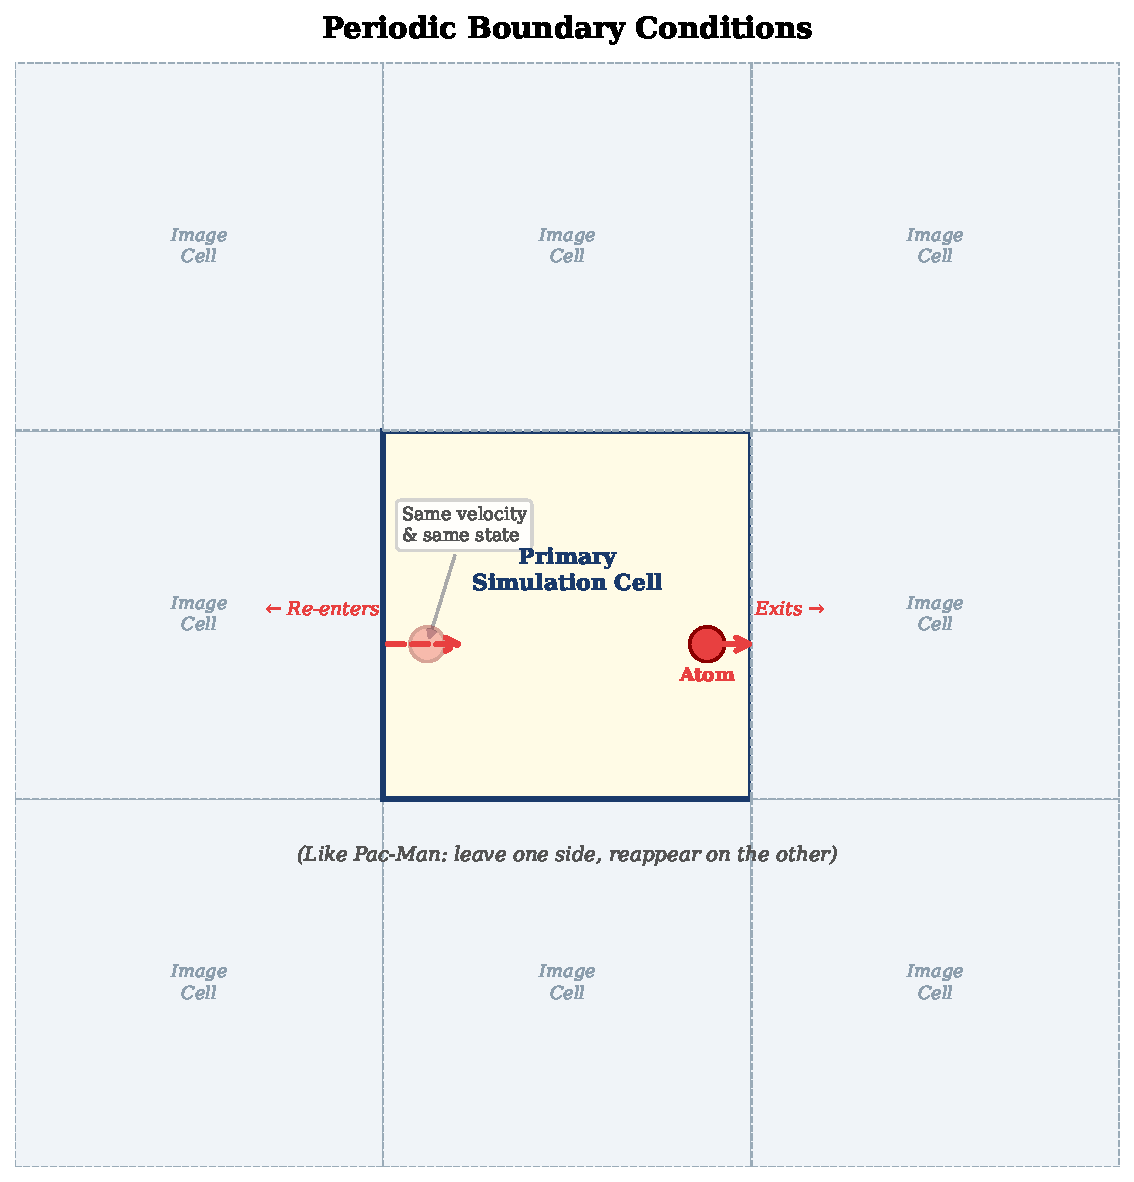
\includegraphics[width=0.72\linewidth]{figures/pbc_schematic.pdf}
    \caption{Periodic Boundary Conditions illustrated in 2D. The central yellow cell is the primary simulation cell; dashed cells are identical image replicas tiling all space. When the red atom exits the right boundary, it immediately re-enters from the left with the same velocity, keeping the total particle count constant. (credit to Claude for the image)}
    \label{fig:pbc}
\end{figure}

\subsubsection{What Is the Minimum Image Convention and Why Do We Apply It?}

Periodic Boundary Conditions solve the surface effect problem, but they introduce a new computational challenge: by definition, PBC creates an infinite array of replica cells extending throughout all of space. Naively, this means every atom in the primary cell must interact with infinitely many copies of every other atom in the universe. Without a system to limit these interactions, the simulation becomes mathematically impossible.

The Minimum Image Convention (MIC) is the \emph{filter} that makes PBC computationally feasible and physically correct. The MIC states a simple rule: when calculating the interaction between any two atoms, use only the \emph{nearest periodic image} of each pair. In practice, this means:

\begin{enumerate}
    \item Calculate the distance vector between atoms $i$ and $j$ in the primary cell.
    \item Apply periodic wrapping: if the distance component along any axis exceeds $L/2$, fold it back across the boundary to find the shortest path through the periodic lattice.
    \item Use this shortest distance to compute the potential energy and forces.
\end{enumerate}

\begin{figure}[H]
    \centering
    \begin{tikzpicture}[scale=1.2]
        % Draw adjacent image cells (dashed)
        \draw[gray!50, dashed] (-6,-2) rectangle (-2,2);
        \draw[gray!50, dashed] (2,-2) rectangle (6,2);
        \node[gray, font=\scriptsize] at (4, -1.7) {Image Cell};
        \node[gray, font=\scriptsize] at (-4, -1.7) {Image Cell};

        % Draw primary central cell (solid)
        \draw[thick, blue!80!black] (-2,-2) rectangle (2,2);
        \node[blue!80!black, font=\scriptsize] at (0, -1.7) {Primary Cell};

        % Box dimension L
        \draw[<->, thick] (-2, -2.3) -- (2, -2.3) node[midway, below] {$L$};

        % Atoms
        \filldraw[blue] (1.2, 0.4) circle (0.1) node[above right] {$i$};
        \filldraw[red] (-1.4, -0.3) circle (0.1) node[above left] {$j$};

        % Image atom
        \filldraw[red!40] (2.6, -0.3) circle (0.1) node[right, font=\small] {image $j'$};

        % Vectors
        \draw[->, red, thick, dashed] (1.2, 0.4) -- (-1.4, -0.3) node[midway, above, sloped, font=\scriptsize] {naive distance};
        \draw[->, green!60!black, thick] (1.2, 0.4) -- (2.6, -0.3) node[midway, below, sloped, font=\scriptsize] {MIC distance};
    \end{tikzpicture}
    \caption{Visualising the Minimum Image Convention (MIC). Atom $i$ interacts with the nearest periodic image $j'$, taking the shortest path across the boundary rather than the longer naive distance to the primary atom $j$.}
    \label{fig:mic_visual}
\end{figure}

A key subtlety: PBC and MIC work together correctly only if the simulation cell is large enough that the periodic images do not interfere with each other. This requires the interaction cutoff $r_c$ to satisfy $r_c \leq L/2$. This is discussed in detain in section \ref{sec:mic_constraint}.

\subsection{How Is It Implemented?}

\subsubsection{Periodic Boundary Wrapping}

After each integration step, any atom whose coordinate has drifted outside $[0, L)$ is wrapped back using the modulo operation:
\begin{equation}
    \mathbf{r}_i \leftarrow \mathbf{r}_i \bmod L
    \label{eq:pbc_wrap}
\end{equation}
This is equivalent to the conditional logic ($x > L \Rightarrow x - L$; $x < 0 \Rightarrow x + L$) but handles arbitrarily large displacements in a single line.

\subsubsection{Minimum Image Convention}
\label{sec:mic}

\begin{equation}
    dx_{ij} = x_i - x_j - L \cdot \mathrm{round}\!\left(\frac{x_i - x_j}{L}\right)
    \label{eq:mic}
\end{equation}
The rounding step identifies which periodic image of atom $j$ is closest to atom $i$ and shifts the distance accordingly. By construction, $dx_{ij} \in (-L/2,\, L/2]$, meaning the result is always the shortest path between the two atoms, whether that path goes through a wall or not.

\subsubsection{Cutoff Constraint}
\label{sec:mic_constraint}

The Minimum Image Convention (MIC) operates on a fundamental assumption: a particle interacts with only the single closest periodic image of any other particle. For this assumption to remain physically valid, the interaction cutoff radius must satisfy:
\begin{equation}
    r_c \leq \frac{L}{2}
    \label{eq:cutoff_constraint}
\end{equation}

If $r_c > L/2$, the physical "sphere of influence" around a particle becomes large enough to span across the periodic boundaries. As illustrated in Figure~\ref{fig:cutoff_constraint}, this causes the cutoff sphere to encompass multiple images of the exact same neighbour. Because the MIC algorithm mathematically truncates the distance to only the single nearest image, any secondary images falling within the $r_c$ range are artificially ignored. This creates a severe physical inconsistency where valid forces are discarded, leading to incorrect dynamics. 

In our simulation, $r_c^* = 2.5$ and the box length is $L^* \approx 6.71$ (for $n_\text{cells} = 4$, $\rho^* = 0.8442$). This yields $L/2 \approx 3.35$. Since $3.35 > 2.5$, the constraint is safely satisfied, ensuring no particle self-interacts or sees multiple images of its neighbours.

\begin{figure}[H]
    \centering
    \begin{tikzpicture}[scale=1.2]
        % Draw adjacent image cells (dashed)
        \draw[gray!50, dashed] (-6,-2) rectangle (-2,2);
        \draw[gray!50, dashed] (2,-2) rectangle (6,2);

        % Draw primary central cell (solid)
        \draw[thick, blue!80!black] (-2,-2) rectangle (2,2);
        \node[blue!80!black, font=\scriptsize] at (0, -1.7) {Primary Cell};

        % Center atom i
        \filldraw[blue] (0.6, 0) circle (0.1) node[above right] {$i$};

        % Atom j and its image
        \filldraw[red] (1.7, 0) circle (0.1) node[right] {$j$};
        \filldraw[red!40] (-2.3, 0) circle (0.1) node[left] {image $j'$};

        % L/2 boundaries
        \draw[<->, gray!80, thick] (-2, -2.3) -- (0, -2.3) node[midway, below, font=\scriptsize] {$L/2$};
        \draw[<->, gray!80, thick] (0, -2.3) -- (2, -2.3) node[midway, below, font=\scriptsize] {$L/2$};

        % Safe cutoff (Green)
        \draw[green!60!black, thick, dashed] (0.6, 0) circle (1.3);
        \draw[->, green!60!black] (0.6,0) -- (0.6, 1.3) node[midway, left, font=\scriptsize] {$r_c$};
        \node[green!60!black, font=\scriptsize, align=center] at (0.6, 1.6) {Safe: $r_c \leq L/2$ \\ (sees $j$ only)};

        % Unsafe cutoff (Red)
        \draw[red, thick, dashed] (0.6, 0) circle (3.1);
        \node[red, font=\scriptsize, align=center] at (0.6, 3.4) {Unsafe: $r_c > L/2$ \\ (sphere overlaps $j$ AND $j'$)};
    \end{tikzpicture}
    \caption{Visualizing the Cutoff Constraint. If the interaction cutoff $r_c$ exceeds $L/2$, the physical interaction sphere around atom $i$ encompasses both the primary atom $j$ and its periodic image $j'$. The MIC algorithm breaks down under these conditions, as it is designed to evaluate only a single unique pair interaction.}
    \label{fig:cutoff_constraint}
\end{figure}
\subsubsection{FCC Lattice Generation}

The simulation box length is determined from the target reduced number density:
\begin{equation}
    L = \left(\frac{N}{\rho^*}\right)^{1/3}, \quad N = 4\,n_\text{cells}^3
    \label{eq:box_length}
\end{equation}
A single FCC unit cell of side $a = L / n_\text{cells}$ contains four atoms at basis positions:
\begin{equation}
    \mathbf{b}_1 = (0,\,0,\,0),\quad
    \mathbf{b}_2 = \tfrac{a}{2}(1,\,1,\,0),\quad
    \mathbf{b}_3 = \tfrac{a}{2}(1,\,0,\,1),\quad
    \mathbf{b}_4 = \tfrac{a}{2}(0,\,1,\,1)
    \label{eq:fcc_basis}
\end{equation}
The full lattice is built by translating this unit cell to all $n_\text{cells}^3$ positions.

\newpage
\subsection{Test Results}

\subsubsection{FCC Lattice: Visualisation}

Figure~\ref{fig:fcc_lattice} shows the FCC lattice generated by \texttt{generate\_fcc\_lattice} with $n_\text{cells} = 3$ and $\rho^* = 4.0$ (a denser packing chosen for visual clarity). The resulting $N = 108$ atoms and box length $L = 3.0$ produce a clear FCC pattern. The characteristic feature of FCC (atoms at face centres offset by $a/2$ from corner atoms) is visible in the regular diagonal arrangements across each face of the cube.

\begin{figure}[H]
    \centering
    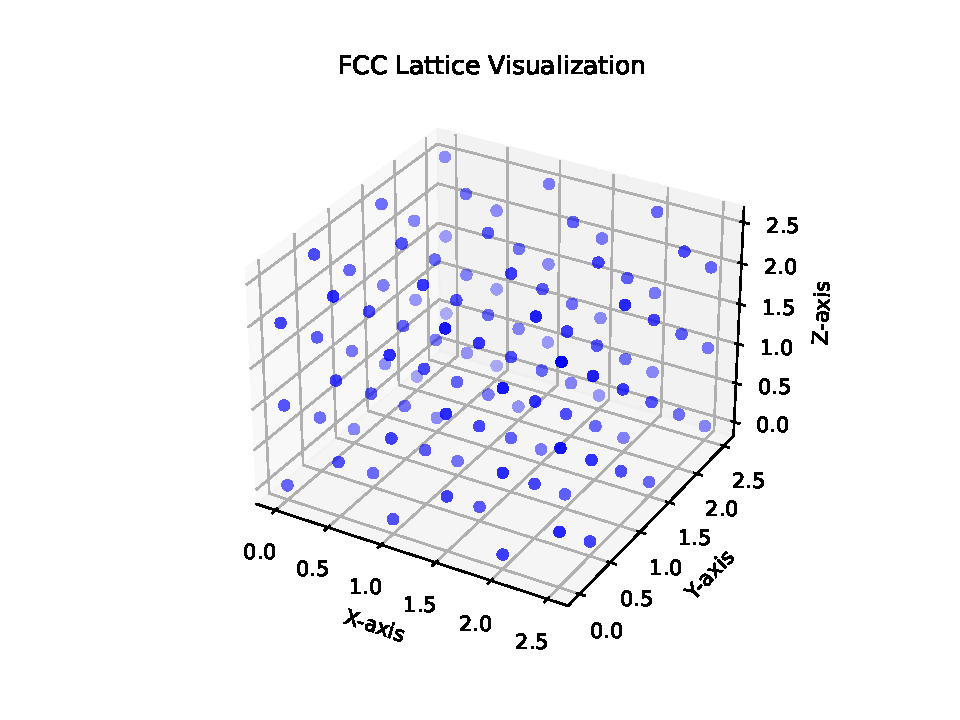
\includegraphics[width=0.62\linewidth]{figures/fcc_lattice.pdf}
    \caption{FCC lattice generated by \texttt{generate\_fcc\_lattice} with $n_\text{cells} = 3$, $\rho^* = 4.0$, giving $N = 108$ atoms in a box of $L = 3.0\,\sigma$. }
    \label{fig:fcc_lattice}
\end{figure}

To further verify the structural integrity of the generated geometry, orthogonal planar projections of the lattice onto the XY, YZ, and ZX planes are presented in Figure~\ref{fig:fcc_projections}. When an FCC structure is viewed precisely along any principal axis, the combination of corner and face-centred atoms aligns to form a regular 2D square grid with a spacing of exactly half the lattice constant ($a/2$). For our system with $L = 3.0$ and $n_\text{cells} = 3$, the lattice constant is $a = 1.0$. The projections correctly demonstrate atoms appearing at precise $0.5$ intervals along all axes, confirming the accurate spatial distribution and periodic boundaries of the setup.

\begin{figure}[H]
    \centering
    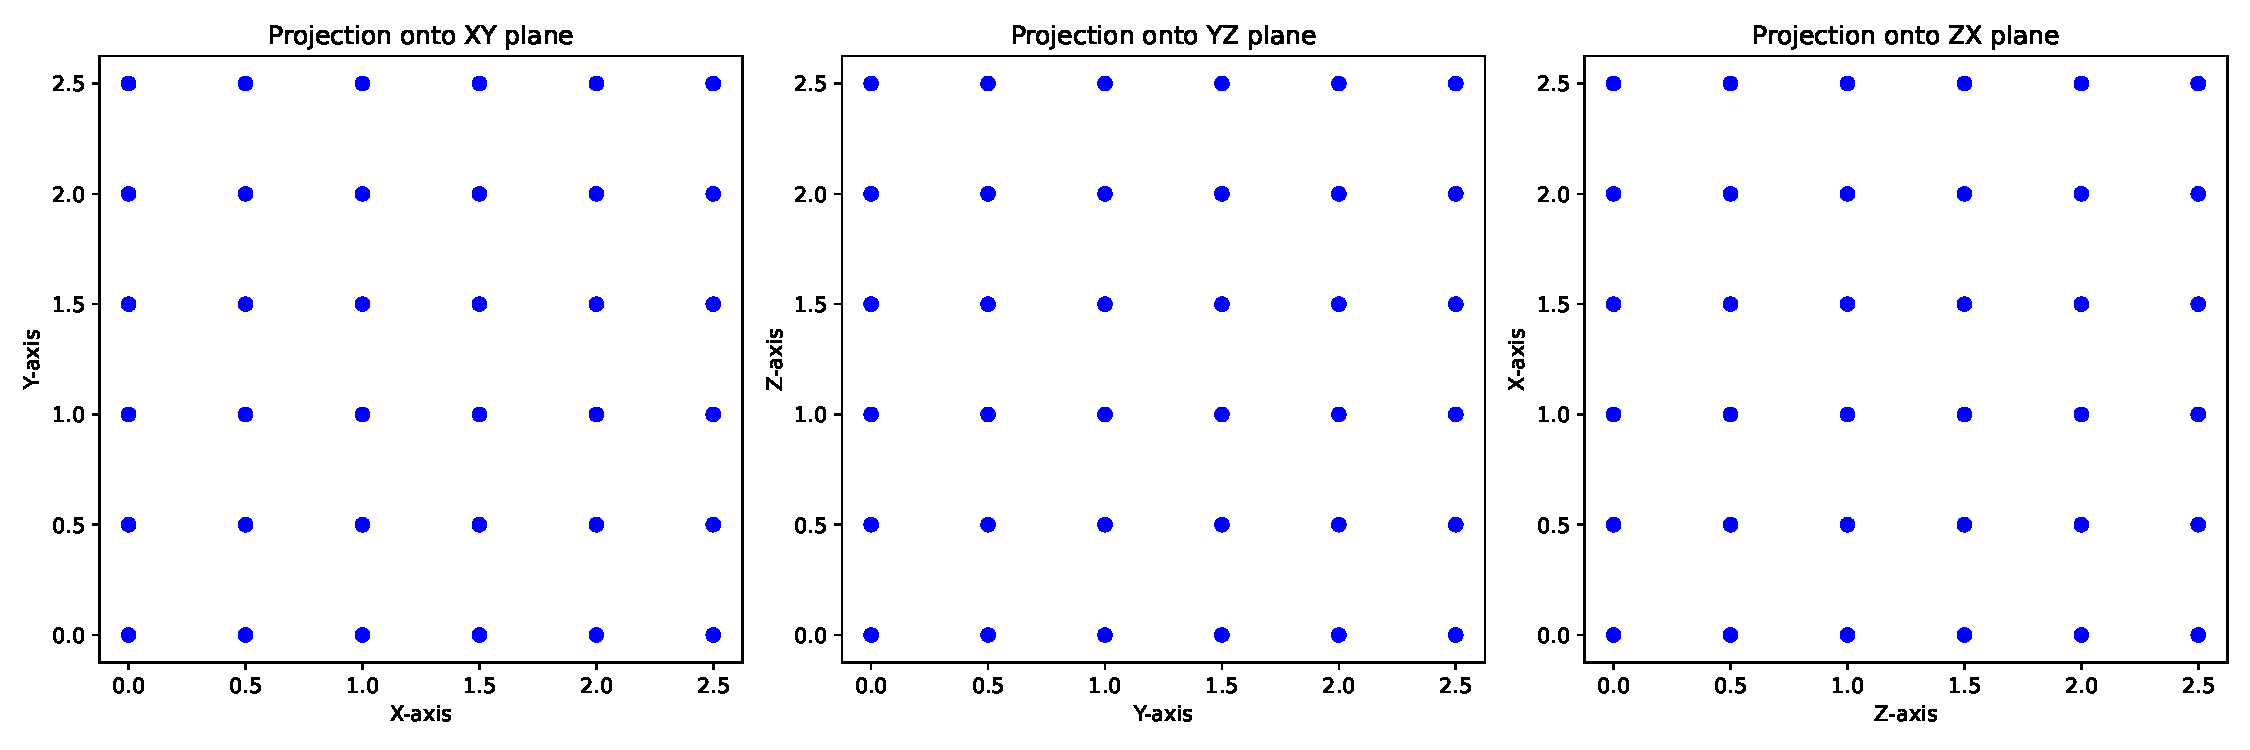
\includegraphics[width=\linewidth]{figures/fcc_lattice_2d_projection.pdf}
    \caption{Orthogonal projections of the simulated FCC lattice onto the XY, YZ, and ZX planes. The uniform grid with spacing $0.5\,\sigma$ confirms the correct structural implementation and the characteristic $a/2$ atomic offsets of the face-centred cubic geometry.}
    \label{fig:fcc_projections}
\end{figure}


\subsubsection{Minimum Image Convention: Visualisation and Test}
\label{sec:mic_test}

Figure~\ref{fig:mic} illustrates the application of the \texttt{apply\_minimum\_image} algorithm in a 2D system, verifying its ability to correctly fold coordinates across periodic boundaries.

In this test case, the simulation box has a length of $L = 10$, spanning from $0$ to $10$ along both axes. Atom 1 (the reference atom, shown in blue) is located at the center $\mathbf{r}_1 = (5, 5)$. Atom 2 (shown in red) has a raw coordinate of $\mathbf{r}_2 = (11, 4)$, placing it completely outside the primary simulation box.

The naive, direct displacement vector from Atom 1 to Atom 2 is:
\begin{equation*}
    \Delta\mathbf{r}_{\text{raw}} = \mathbf{r}_2 - \mathbf{r}_1 = (11 - 5, 4 - 5) = (6, -1)
\end{equation*}

Because the magnitude of the $x$-displacement ($\Delta x = 6$) is strictly greater than $L/2 = 5$, it violates the minimum image criteria. The MIC algorithm corrects this by applying the rounding formula to find the shortest path across the periodic boundary:
\begin{equation*}
    dx_{\text{MIC}} = 6 - 10 \cdot \mathrm{round}\left(\frac{6}{10}\right) = 6 - 10 \times 1 = -4
\end{equation*}
The $y$-displacement ($\Delta y = -1$) is already within the $[-5, 5]$ bounds, so it remains unchanged ($dy_{\text{MIC}} = -1 - 10 \times 0 = -1$). The resulting MIC displacement vector is $\Delta\mathbf{r}_{\text{MIC}} = (-4, -1)$.

As shown in Figure~\ref{fig:mic}, adding this corrected displacement vector to Atom 1 yields the effective position of Atom 2's closest periodic image: $(5, 5) + (-4, -1) = (1, 4)$. The solid green line accurately represents this minimum image distance, confirming that the code successfully maps the atom to its correct periodic representation (the green dot) within the primary interaction neighbourhood.

\begin{figure}[H]
    \centering
    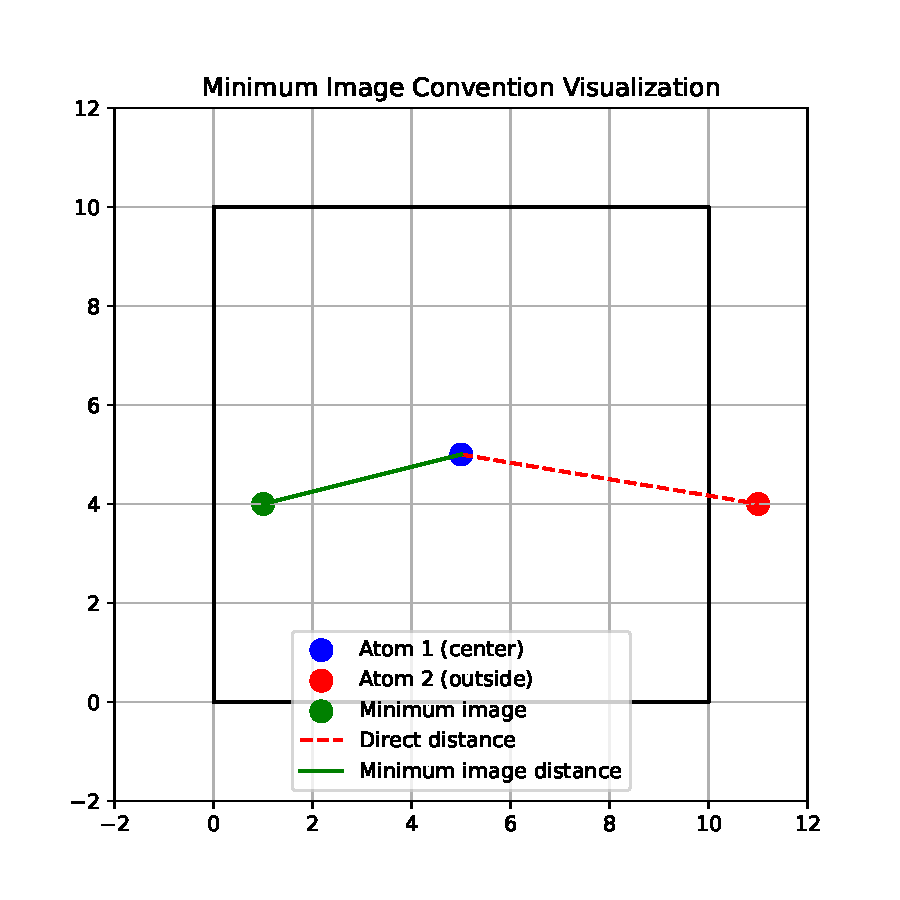
\includegraphics[width=0.8\linewidth]{figures/minimum_image_convention.pdf}
    \caption{Minimum Image Convention (MIC) visualization in a 2D box of $L = 10$. Atom 1 is located at $(5,5)$ and Atom 2 is outside the box at $(11,4)$. The direct distance (dashed red line) yields an $x$-displacement of $6$, exceeding $L/2$. The MIC algorithm folds the calculation across the periodic boundary, correctly identifying the minimum image of Atom 2 at $(1,4)$ (green dot). The solid green line represents the true shortest interaction vector $\Delta\mathbf{r}_{\text{MIC}} = (-4, -1)$ computed by the algorithm.}
    \label{fig:mic}
\end{figure}
% =============================================================
%  SECTION: Module 3 — The Velocity Verlet Integrator
%  ASSIGNED TO: [Person Name]
%
%  GUIDING QUESTIONS TO ANSWER:
%   WHAT  — What is numerical integration? What does Velocity Verlet do?
%   WHY   — Why can't we solve the equations of motion analytically?
%           Why Velocity Verlet over, say, simple Euler integration?
%   HOW   — Walk through the 4-step VV algorithm.
%           How is energy conservation used as a reliability check?
%  EXTRAS — What is a "good" time step? The 1-in-10^4 fluctuation rule.
%           What does energy drift look like when dt is too large?
%           What is the reduced time unit t* and how is dt chosen?
% =============================================================

\newpage
\section{Module 3: The Velocity Verlet Integrator}

\subsection{What Are We Doing?}
% We need to evolve atomic positions and velocities forward in time.
% Since forces change constantly, there's no closed-form solution → finite differences.
% [WRITE HERE]

\subsection{Why Are We Doing It?}

\subsubsection{Why Can't We Solve This Analytically?}
% N coupled, nonlinear ODEs. Positions affect forces, forces affect positions.
% No analytical solution for N > 2. Must discretise time.
% [WRITE HERE]

\subsubsection{Why Velocity Verlet?}
% Compare to simple Euler: VV is time-reversible, symplectic (conserves phase volume),
% and synchronises positions and velocities at the same time step.
% Euler accumulates error; VV oscillates around the true energy without drift.
% [WRITE HERE — intuition is key here]

\subsection{How Is It Implemented?}

\subsubsection{The Algorithm}

The Velocity Verlet update proceeds in four steps per timestep $\delta t^*$:

\begin{enumerate}
    \item \textbf{Update positions:}
    \begin{equation}
        \mathbf{r}_i(t+\delta t) = \mathbf{r}_i(t) + \mathbf{v}_i(t)\,\delta t + \tfrac{1}{2}\mathbf{a}_i(t)\,\delta t^2
        \label{eq:vv_pos}
    \end{equation}

    \item \textbf{Half-step velocity:}
    \begin{equation}
        \mathbf{v}_i\!\left(t + \tfrac{1}{2}\delta t\right) = \mathbf{v}_i(t) + \tfrac{1}{2}\mathbf{a}_i(t)\,\delta t
        \label{eq:vv_vhalf}
    \end{equation}

    \item \textbf{Recalculate forces} from new positions (Module 1 + 2 logic).

    \item \textbf{Complete velocity update:}
    \begin{equation}
        \mathbf{v}_i(t + \delta t) = \mathbf{v}_i\!\left(t + \tfrac{1}{2}\delta t\right) + \tfrac{1}{2}\mathbf{a}_i(t+\delta t)\,\delta t
        \label{eq:vv_vfull}
    \end{equation}
\end{enumerate}

In reduced units, $m^* = 1$, so $\mathbf{a}_i^* = \mathbf{F}_i^*$.

\subsubsection{Choosing the Time Step}

The reduced time unit is $t^* = t/t_0$ where $t_0 = \sigma\sqrt{m/\eps}$. A good rule of thumb is to have $\sim50$ timesteps per vibrational period. For the LJ system we use $\delta t^* = 0.005$. The stability criterion is:
\begin{equation}
    \frac{\Delta E^*}{\langle E^* \rangle} \lesssim 10^{-4}
\end{equation}
where $\Delta E^*$ is the fluctuation in total energy during the production run.

\subsubsection{Kinetic and Potential Energy}

In reduced units ($m^* = 1$):
\begin{align}
    K^* &= \frac{1}{2}\sum_{i=1}^{N} |\mathbf{v}_i^*|^2 \label{eq:ke}\\
    E^* &= K^* + U^* \label{eq:etot}
\end{align}

\subsection{Test Results}

% Run a short simulation (e.g. 200 steps) of a 2-atom or 32-atom system.
% Plot E*, K*, U* vs time step.
% Confirm total energy is flat (no drift), KE and PE oscillate but compensate.

\begin{figure}[H]
    \centering
    % 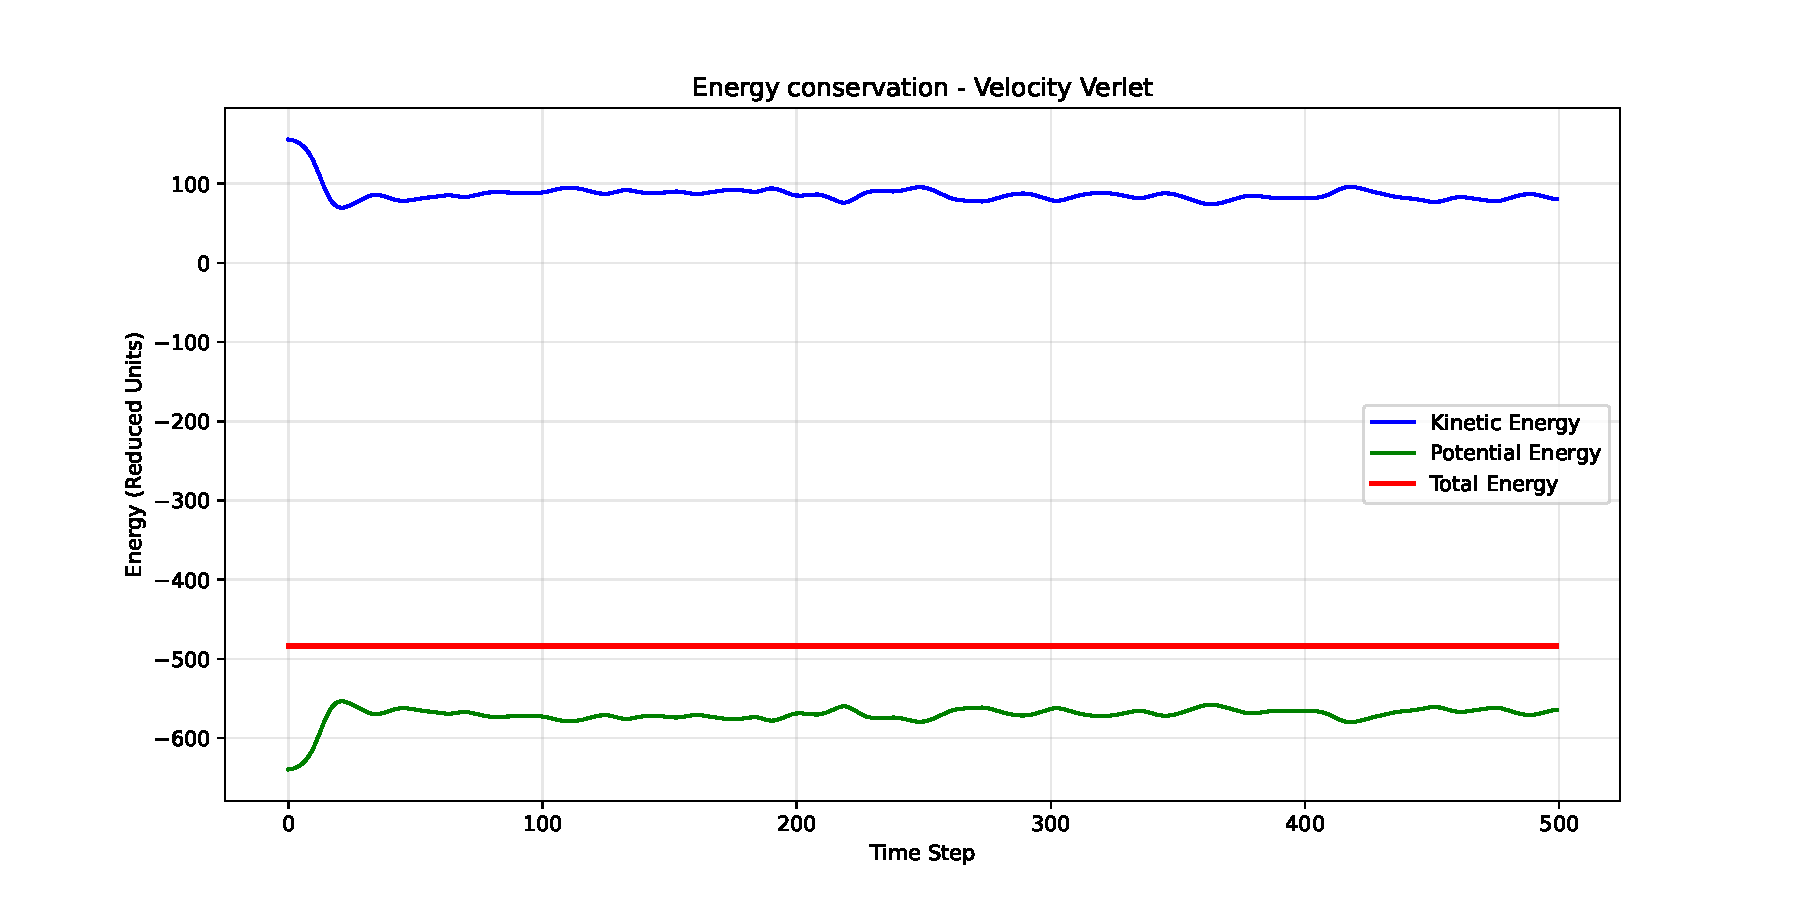
\includegraphics[width=\linewidth]{figures/m3_energy_conservation.pdf}
    \caption{Total energy $E^*$, kinetic energy $K^*$, and potential energy $U^*$ over time for a test run using the Velocity Verlet integrator with $\delta t^* = 0.005$. The total energy shows no systematic drift, confirming the integrator is working correctly.}
    \label{fig:m3_energy}
\end{figure}

% Report: mean E*, standard deviation of E*, ratio std/mean (should be ~1e-4 or better).
% [WRITE QUANTITATIVE RESULTS HERE]

% =============================================================
%  SECTION: Module 4 — Performance and Optimization
%  ASSIGNED TO: [Person Name]
%
%  GUIDING QUESTIONS TO ANSWER:
%   WHAT  — What is the O(N²) bottleneck? What is a Verlet neighbor list?
%           What is NumPy vectorization?
%   WHY   — Why does the naive force loop become a problem at N=500?
%           Why does the skin radius allow infrequent rebuilds?
%           Why does the shifted force potential improve energy conservation?
%   HOW   — How is the neighbor list built? When is it rebuilt?
%           How does vectorization replace Python for-loops?
%  EXTRAS — Benchmark: show timing comparison naive vs optimized (optional).
%           Explain the shifted-force potential and how it differs from
%           the shifted potential in Module 1.
% =============================================================

\newpage
\section{Module 4: Performance and Optimization}

\subsection{What Are We Doing?}
% Refactoring the force calculation to (1) skip distant pairs using a neighbor
% list, and (2) use NumPy array operations instead of Python loops.
% [WRITE HERE]

\subsection{Why Are We Doing It?}

\subsubsection{The \texorpdfstring{$O(N^2)$}{O(N²)} Bottleneck}
% With N atoms, naive force loop: N*(N-1)/2 pair checks per step.
% For N=500: ~125,000 checks every timestep. Most are beyond r_c and contribute zero.
% Show or cite the scaling: double N → 4x slower.
% [WRITE HERE]

\subsubsection{Why Does the Skin Radius Work?}
% Atoms move slowly relative to r_skin - r_c.
% Only rebuild when max displacement > (r_skin - r_c)/2.
% Analogy: you don't update your contact list every second — only when someone moves.
% [WRITE HERE — good place for physical intuition]

\subsubsection{Why the Shifted-Force Potential?}
% Even with a shifted potential, the force magnitude has a jump at r_c.
% This jump acts as a source/sink of energy every time a pair crosses the boundary.
% The shifted-force potential sets both phi and F smoothly to zero at r_c.
% [WRITE HERE]

\subsection{How Is It Implemented?}

\subsubsection{Verlet Neighbor List}

All pairs $(i, j)$ with separation $r_{ij} < r_s$ are stored, where the skin radius is:
\begin{equation}
    r_s = r_c + \delta_{\text{skin}}
    \label{eq:rskin}
\end{equation}
We used $r_c^* = 2.5$ and $r_s^* = 3.2$, giving a skin thickness of $0.7\,\sigma$.

The list is rebuilt only when any atom has displaced more than half the skin thickness from its last recorded position:
\begin{equation}
    \Delta r_{\max} > \frac{r_s - r_c}{2}
    \label{eq:rebuild}
\end{equation}

\subsubsection{The Shifted-Force Potential}

To ensure both energy and force vanish at $r_c$:
\begin{equation}
    \phi_{\text{SF}}^*(r^*) = \phi^*(r^*) - \phi^*(r_c^*) + \left.\frac{d\phi^*}{dr^*}\right|_{r_c^*}\!\!(r^* - r_c^*)
    \label{eq:shifted_force}
\end{equation}

% [EXPLAIN IN WORDS — what does subtracting the linear term do?]

\subsubsection{NumPy Vectorization}

Instead of nested loops, all pair displacements are computed simultaneously using broadcast array operations, reducing Python-level overhead by orders of magnitude.

\subsection{Test Results}

% Confirm:
% 1. The optimized force routine gives identical energies to the naive version (for small N).
% 2. Show how often the neighbor list is rebuilt (e.g., every ~X steps).
% 3. (Optional) timing comparison: naive loop vs. vectorized.

% [INSERT RESULTS / TIMING TABLE HERE]

\begin{table}[H]
    \centering
    \caption{Comparison of naive and optimized force calculation for $N = 256$ atoms.}
    \label{tab:m4_timing}
    \begin{tabular}{lcc}
        \toprule
        \textbf{Method} & \textbf{Time per step (ms)} & \textbf{Energy match?} \\
        \midrule
        Naive (all pairs) & [value] & --- \\
        Neighbor list + vectorized & [value] & [Yes/No] \\
        Speedup factor & [ratio] & \\
        \bottomrule
    \end{tabular}
\end{table}

% [WRITE DISCUSSION HERE]

% =============================================================
%  SECTION: Module 5 — Initialization, Equilibration & Assembly
%  ASSIGNED TO: [Person Name]
%
%  GUIDING QUESTIONS TO ANSWER:
%   WHAT  — What is the Maxwell-Boltzmann distribution?
%           What is velocity rescaling? What is equilibration?
%   WHY   — Why can't we just give all atoms the same speed?
%           Why zero the net momentum before running?
%           Why run an equilibration phase before collecting data?
%   HOW   — How is Gaussian sampling used to initialise velocities?
%           How does the rescaling thermostat work (lambda factor)?
%           What are the equilibration and production phases?
%  EXTRAS — Energy compensation: K* and U* oscillate anti-phase.
%           Plot of K*, U*, E* all on one graph.
%           What happens to E* during equilibration vs production?
% =============================================================
% =============================================================
%  SECTION: Module 5 — Initialization, Equilibration & Assembly
% =============================================================

\newpage
\section{Module 5: Initialization, Equilibration, and System Assembly}

\subsection{What Are We Doing?}

Having built the tools to compute forces (Module 1), enforce periodic geometry (Module 2), propagate motion (Module 3), and do so efficiently (Module 4), we are now ready to assemble them into a working simulation. But before the engine can run, we must answer two questions that every real physicist faces when setting up an experiment: \emph{how do we prepare the system in a physically valid state?} and \emph{how long do we wait before we trust any measurement?}

This module solves both problems. It assigns every atom a velocity drawn from the correct statistical distribution for the target temperature, eliminates any spurious centre-of-mass drift, and then runs an equilibration phase — a controlled warm-up period — before the simulation settles into the stable state from which we collect data.

\subsection{Why Are We Doing It?}

\subsubsection{Why Maxwell-Boltzmann Velocities?}

Imagine you are running at a temperature $T^*$ and you need to assign each atom a starting speed. The naive approach — give every atom exactly the same speed — creates an artificial, crystalline structure in velocity space that does not resemble any real material. In reality, atoms in thermal equilibrium do not move uniformly. Some are slow, some are fast, and their speeds span a continuous range set by the \textbf{Maxwell-Boltzmann distribution} — a direct consequence of classical statistical mechanics.

This distribution tells us that each individual velocity component ($v_x$, $v_y$, $v_z$) of any given atom is a Gaussian random variable with zero mean and a spread determined entirely by temperature. In reduced units, the standard deviation is simply $\sigma = \sqrt{T^*}$: hotter systems have faster, more spread-out velocity distributions. By sampling each component from this Gaussian, we start the simulation as close as possible to a real thermal equilibrium — no artificial symmetry, no unphysical ordering.

\subsubsection{Why Zero the Net Momentum?}

When $N$ velocities are drawn at random from a Gaussian, the sum will not be exactly zero — statistical fluctuations guarantee a small, nonzero net momentum $\mathbf{P}^* = \sum_i \mathbf{v}_i$. This is harmless in nature (where there is no preferred reference frame), but in a simulation it is catastrophic. A nonzero total momentum means the entire collection of atoms is slowly drifting in one direction, as if the whole simulation box were a single projectile. Over time, atoms leave one side of the periodic cell faster than they re-enter from the other, breaking the statistical homogeneity that makes PBC valid.

The fix is one line: subtract the mean velocity from every atom before the simulation begins. This zeroes $\mathbf{P}^*$ exactly and anchors the centre of mass permanently to rest.

\subsubsection{Why an Equilibration Phase?}

We begin on a perfect FCC lattice — every atom sitting precisely at its ideal lattice site, none of them where they would actually be in a thermodynamically equilibrated solid or liquid. This is a highly artificial initial condition: the atoms have not yet had time to settle into their natural configurations, and the kinetic and potential energies are far from their equilibrium balance.

If we were to start collecting data immediately, every measurement would be contaminated by this transient. The $g(r)$ would reflect the perfect FCC geometry rather than true thermal structure; the energy would still be drifting toward its equilibrium value. The equilibration phase gives the system time to relax: we run the integrator while periodically forcing the temperature back to its target value, letting the atoms reorganise while guiding the system toward equilibrium. Once the energies have settled into steady oscillations and the temperature is stable, we switch off the thermostat and let the system run freely — this is the production phase, and only now do we trust the data.

\subsection{How Is It Implemented?}

\subsubsection{Velocity Initialization}

Each velocity component $v_{i\alpha}$ is sampled independently from a Gaussian:
\begin{equation}
    \rho(v_{i\alpha}) = \frac{1}{\sigma\sqrt{2\pi}}\exp\!\left(-\frac{v_{i\alpha}^2}{2\sigma^2}\right),
    \quad \sigma = \sqrt{\Tstar}
    \label{eq:mb}
\end{equation}
After sampling, the mean velocity is subtracted component-wise so that $\sum_i \mathbf{v}_i = \mathbf{0}$ exactly. In our test run, the residual momentum after this step was $|\mathbf{P}^*| = 1.77 \times 10^{-14}$ — numerical noise at the level of floating-point precision.

\subsubsection{Velocity Rescaling Thermostat}

At any instant during the simulation, the instantaneous reduced temperature is directly related to the total kinetic energy:
\begin{equation}
    \Tstar_{\text{inst}} = \frac{1}{3N}\sum_i |\mathbf{v}_i^*|^2
    \label{eq:T_inst}
\end{equation}
To steer the system toward a target $\Tstar_{\text{target}}$, all velocities are multiplied by a single scaling factor $\lambda$:
\begin{equation}
    \lambda = \sqrt{\frac{\Tstar_{\text{target}}}{\Tstar_{\text{inst}}}}
    \qquad\Rightarrow\qquad
    \mathbf{v}_i^{\text{new}} = \lambda\,\mathbf{v}_i
    \label{eq:rescale}
\end{equation}
This works because kinetic energy scales as $v^2$: multiplying every speed by $\lambda$ multiplies $K^*$ by $\lambda^2 = T_{\text{target}}/T_{\text{inst}}$, exactly reaching the target. Rescaling is applied every 10 steps during the equilibration phase; it is switched off entirely during production so the system evolves freely in the NVE ensemble.

\subsubsection{The Master MD Loop}

The complete simulation proceeds in three stages:

\begin{enumerate}
    \item \textbf{Initialise:} Generate the FCC lattice (Module 2), assign Maxwell-Boltzmann velocities, zero net momentum, build the initial Verlet neighbour list (Module 4), and compute the initial forces.
    \item \textbf{Equilibration} (steps 0 to $N_{\text{equil}}$): Advance with the Velocity Verlet integrator (Module 3 via Module 4); apply velocity rescaling every 10 steps to hold $T^* \approx T_{\text{target}}$. No data is recorded.
    \item \textbf{Production} (steps $N_{\text{equil}}$ to $N_{\text{total}}$): Thermostat is switched off. The system evolves freely; all energies, temperatures, and structural observables are accumulated.
\end{enumerate}

In this module test we ran $N_{\text{total}} = 5000$ steps with a 50/50 equilibration-to-production split: 2500 equilibration steps followed by 2500 production steps.

\subsection{Energy Compensation: A Key Diagnostic}

As the system relaxes from the perfect FCC lattice during equilibration, the potential and kinetic energies exchange rapidly — $K^*$ rises when atoms fly apart as the lattice melts thermally, and $U^*$ falls correspondingly. These fluctuations are not noise; they are the fundamental exchange between kinetic and potential energy that every classical system undergoes. The critical test is whether they cancel: in a physically correct simulation, every joule that leaves $U^*$ must appear in $K^*$ and vice versa, keeping $E^* = K^* + U^*$ flat. During equilibration, the periodic velocity rescaling will cause visible step-like jumps in $E^*$ as kinetic energy is injected or removed. These jumps vanish completely once the thermostat is switched off and production begins.

\begin{figure}[H]
    \centering
    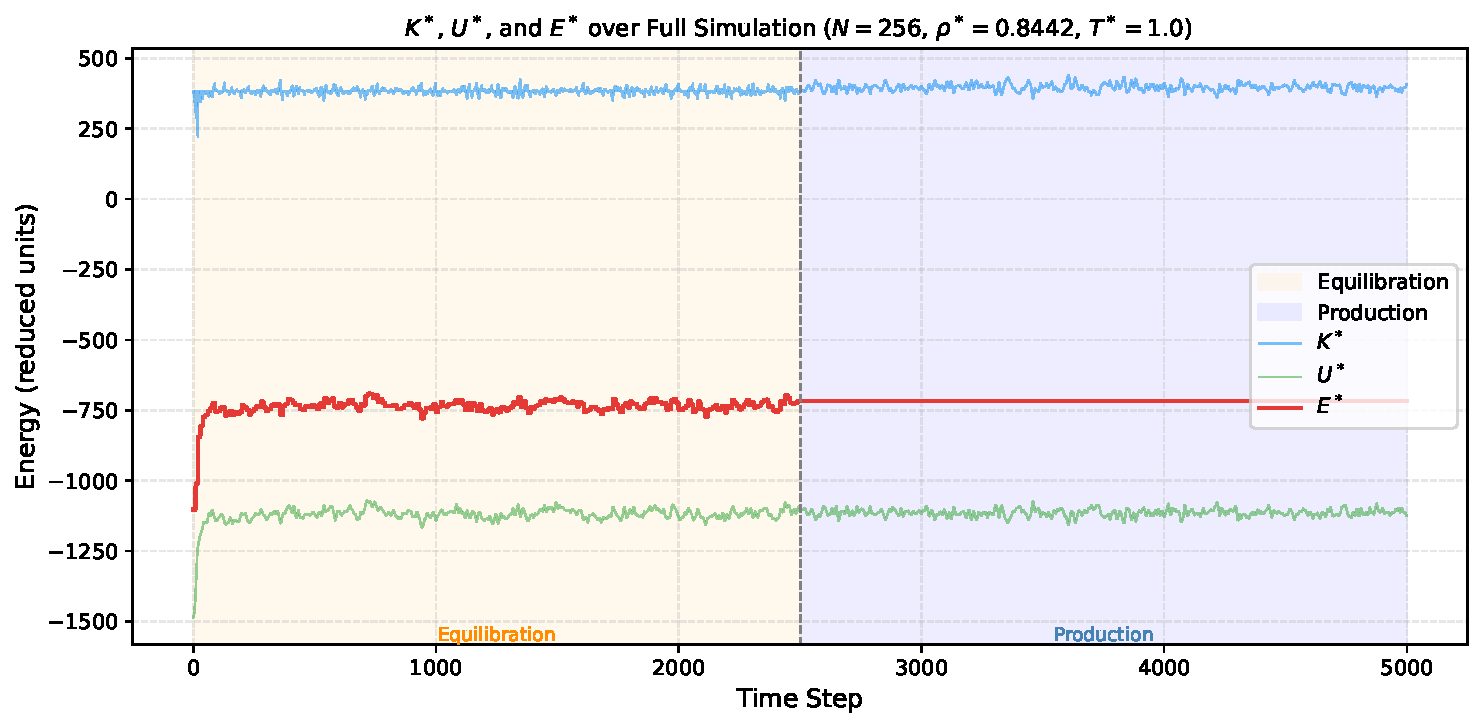
\includegraphics[width=\linewidth]{figures/m5_energy_three_panel.pdf}
    \caption{Kinetic energy $K^*$, potential energy $U^*$, and total energy $E^*$ over all 5000 timesteps for $N=256$, $\rho^* = 0.8442$, $T^* = 1.0$, $\delta t^* = 0.005$. The orange-shaded region is the equilibration phase (steps 0--2500), where velocity rescaling periodically adjusts $K^*$; the blue-shaded region is the production phase (steps 2500--5000), where all quantities evolve freely. The flatness of $E^*$ (red) in the production phase is the primary confirmation of physical correctness.}
    \label{fig:m5_energy}
\end{figure}

\begin{figure}[H]
    \centering
    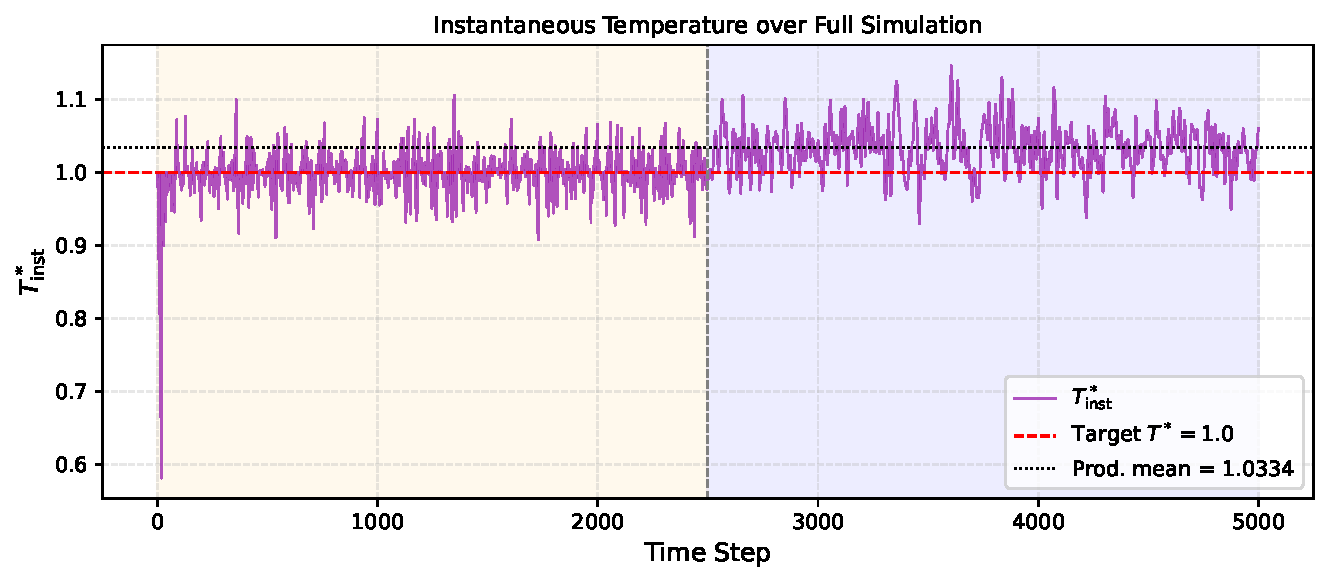
\includegraphics[width=0.9\linewidth]{figures/m5_temperature.pdf}
    \caption{Instantaneous reduced temperature $T^*_\text{inst}$ over all 5000 timesteps. During equilibration the thermostat clamps the temperature tightly to the target $T^* = 1.0$ (red dashed); in production it fluctuates naturally around $\langle T^* \rangle = 1.033$ (black dotted), a small deviation from 1.0 that reflects the finite-size statistical nature of the NVE ensemble after thermostat removal.}
    \label{fig:m5_temp}
\end{figure}

\subsection{Test Results}

\begin{table}[H]
    \centering
    \caption{Module 5 verification for $N = 256$, $\rhostar = 0.8442$, $\Tstar = 1.0$, $\delta t^* = 0.005$, 5000 total steps (2500 equilibration + 2500 production).}
    \label{tab:m5_test}
    \begin{tabular}{lcc}
        \toprule
        \textbf{Quantity} & \textbf{Expected} & \textbf{Measured} \\
        \midrule
        $\langle \Tstar \rangle$ (production)              & $\approx 1.0$         & $1.033$ \\
        Initial $|\mathbf{P}^*|$ after zeroing             & $\approx 0$           & $1.77 \times 10^{-14}$ \\
        Max $|P_x^*|$ during run                           & $\approx 0$           & $1.49 \times 10^{-13}$ \\
        Max $|P_y^*|$ during run                           & $\approx 0$           & $1.16 \times 10^{-13}$ \\
        Max $|P_z^*|$ during run                           & $\approx 0$           & $1.57 \times 10^{-13}$ \\
        $\langle \Estar \rangle$ (production)              & ---                   & $-717.16$ \\
        RMS fluctuation $\Delta \Estar$                    & ---                   & $5.34 \times 10^{-2}$ \\
        Relative fluctuation $\Delta \Estar/|\langle \Estar \rangle|$ & $\lesssim 10^{-4}$ & $7.45 \times 10^{-5}$ \\
        Criterion met?                                      & ---                   & \textbf{Yes} \\
        \bottomrule
    \end{tabular}
\end{table}

All three diagnostic criteria are satisfied. The total momentum components remain at machine-precision levels ($\sim 10^{-13}$) throughout the entire run — they never grow, confirming that the momentum-zeroing step and the Velocity Verlet integrator both preserve $\mathbf{P}^* = \mathbf{0}$ exactly. The relative energy fluctuation of $7.45 \times 10^{-5}$ falls below the $10^{-4}$ threshold, confirming that $\delta t^* = 0.005$ is a stable choice. The production-phase temperature of $\langle T^* \rangle = 1.033$ sits slightly above the target of $1.0$; this is expected and physically correct — once the rescaling thermostat is removed, the NVE ensemble conserves energy rather than temperature, and finite-size fluctuations allow the mean temperature to settle at a value slightly different from the target. The system is in equilibrium, and production data is trustworthy.
% =============================================================
%  SECTION: Module 6 — Radial Distribution Function
%  ASSIGNED TO: [Person Name]
%
%  GUIDING QUESTIONS TO ANSWER:
%   WHAT  — What is g(r)? What does it measure physically?
%   WHY   — Why can't temperature alone tell us if a system is solid or liquid?
%           Why must we normalise by the shell volume and density?
%           Why must g(r) → 1.0 at large r?
%   HOW   — How is the histogram binned? How is the normalization applied?
%           What is the MIC used for in this context?
%  EXTRAS — What do sharp peaks vs. broad/decaying peaks mean physically?
%           Statistical binning: why average over multiple frames?
% =============================================================

\newpage
\section{Module 6: Radial Distribution Function}

\subsection{What Are We Doing?}
% We need a structural metric to distinguish solid from liquid.
% g(r) gives the probability of finding an atom at distance r from a central atom,
% relative to a uniform ideal gas.
% [WRITE HERE]

\subsection{Why Are We Doing It?}

\subsubsection{Why Isn't Temperature Enough?}
% A glass and a liquid can be at the same temperature.
% Structure (how atoms are arranged) is distinct from thermodynamics.
% We need to look at the spatial correlations between atoms.
% [WRITE HERE — build intuition]

\subsubsection{Why Does \texorpdfstring{$g(r) \to 1$}{g(r)→1} at Large \texorpdfstring{$r$}{r}?}
% At large distances, correlations die out. The probability of finding an atom
% is just the bulk density. Dividing by the ideal gas density gives 1.0.
% If g(r) doesn't reach 1.0, the normalization or the simulation is wrong.
% [WRITE HERE]

\subsubsection{What Do the Peaks Tell Us?}

\begin{description}
    \item[Solid:] Sharp, narrow peaks at well-defined distances corresponding to the coordination shells of the FCC lattice. Long-range order persists.
    \item[Liquid:] A prominent first peak (nearest-neighbour shell), then broad, decaying oscillations that quickly reach 1.0, indicating short-range order only.
\end{description}

% [ADD PHYSICAL INTUITION — what is the first peak? second peak?]

\subsection{How Is It Implemented?}

\subsubsection{Algorithm}

\begin{equation}
    g(r) = \frac{V}{4\pi r^2 \Delta r \, N^2}
    \left\langle \sum_i \sum_{j \neq i} \mathbf{1}\!\left[r < r_{ij} < r + \Delta r\right] \right\rangle
    \label{eq:gr}
\end{equation}

\begin{enumerate}
    \item For each snapshot, loop over all unique pairs $(i,j)$ and compute $r_{ij}$ using the MIC.
    \item Bin each $r_{ij}$ into a histogram with bin width $\Delta r$ and up to $r_{\max} = L/2$.
    \item Normalise each bin $k$ (centre $r_k$) by the shell volume and number density:
    \begin{equation}
        g(r_k) = \frac{2 \cdot \text{count}(k) \cdot L^3}{N^2 \cdot 4\pi r_k^2 \Delta r}
        \label{eq:gr_norm}
    \end{equation}
    \item Average $g(r)$ over multiple uncorrelated snapshots from the production run.
\end{enumerate}

\subsubsection{Binning for Statistical Reliability}

Because consecutive MD timesteps are highly correlated, $g(r)$ is collected every 10 steps and the results are averaged. This reduces noise without requiring prohibitively long runs.

\subsection{Test Results}

% Test on a snapshot from the production run.
% Confirm: g(r) → 1.0 at large r (normalization correct).
% Confirm: first peak is near the LJ minimum at r* ≈ 1.12.

\begin{figure}[H]
    \centering
    % 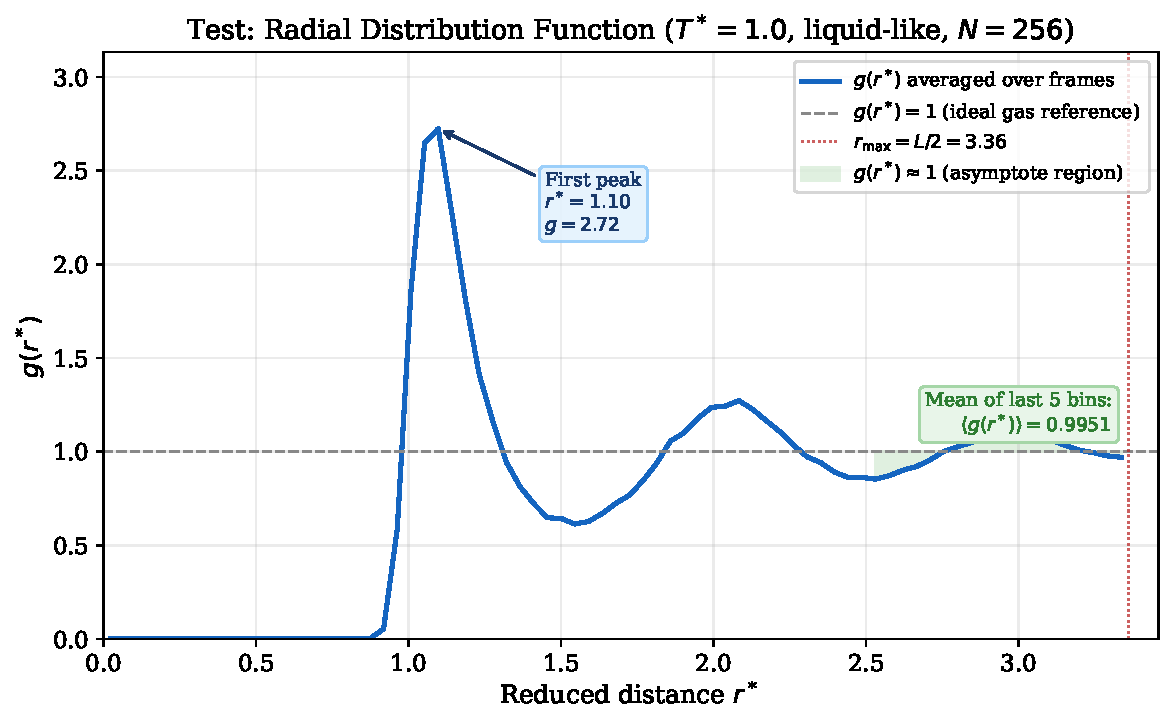
\includegraphics[width=0.75\linewidth]{figures/m6_gr_test.pdf}
    \caption{Test $g(r)$ plot from Module 6, computed on a single production snapshot. The function asymptotes to $g(r) = 1$ (dashed line) at large $r$, confirming correct normalisation.}
    \label{fig:m6_gr_test}
\end{figure}

% [WRITE DISCUSSION OF TEST RESULTS HERE]


% =============================================================
%  PART II: INTEGRATED ENGINE AND DIAGNOSTICS
% =============================================================
\newpage
\part*{Integrated Engine \& Diagnostic Analysis}
\addcontentsline{toc}{part}{Integrated Engine \& Diagnostic Analysis}

% =============================================================
%  SECTION 7, Integrated MD Engine
% ============================================================

\section{Integrated MD Engine}

\subsection{Putting It All Together}

"Each of the six modules was independently built and tested before being integrated into a single working simulation. The core engine is implemented as a single Python class, \texttt{MDSimulation}. This class maintains the complete simulation state, including positions, velocities, forces, and the Verlet neighbour list, and orchestrates the execution of each module in the correct sequence.

\subsection{How the Modules Connect}

The simulation is executed in three distinct phases: initialisation, an equilibration loop, and a production loop. While Figure~\ref{fig:md_flowchart} maps the high-level data routing between modules, the specific physical constraints and parameters applied during each phase are detailed below.

\begin{figure}[H]
\centering
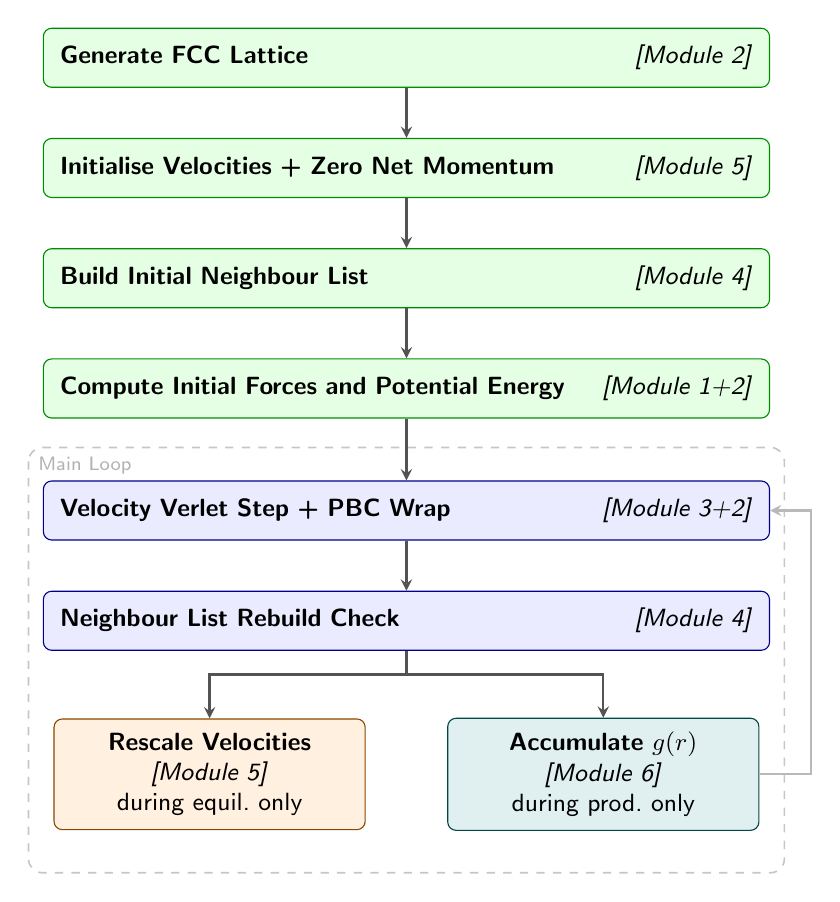
\begin{tikzpicture}[
    ibox/.style = {
        draw, rounded corners=3pt,
        fill=green!10, draw=green!55!black,
        text width=8.8cm, minimum height=0.75cm,
        align=left, inner sep=6pt, font=\small\sffamily
    },
    lbox/.style = {
        draw, rounded corners=3pt,
        fill=blue!8, draw=blue!55!black,
        text width=8.8cm, minimum height=0.75cm,
        align=left, inner sep=6pt, font=\small\sffamily
    },
    ebox/.style = {
        draw, rounded corners=3pt,
        fill=orange!12, draw=orange!55!black,
        text width=3.6cm, minimum height=1.4cm,
        align=center, inner sep=5pt, font=\small\sffamily
    },
    pbox/.style = {
        draw, rounded corners=3pt,
        fill=teal!12, draw=teal!55!black,
        text width=3.6cm, minimum height=1.4cm,
        align=center, inner sep=5pt, font=\small\sffamily
    },
    arr/.style = {->, thick, >=stealth, color=gray!65!black}
]

%% ---- INITIALISATION ----
\node[ibox] (fcc)  at (0,  0.0) {\textbf{Generate FCC Lattice} \hfill \textit{[Module 2]}};
\node[ibox] (vel)  at (0, -1.4) {\textbf{Initialise Velocities + Zero Net Momentum} \hfill \textit{[Module 5]}};
\node[ibox] (nb0)  at (0, -2.8) {\textbf{Build Initial Neighbour List} \hfill \textit{[Module 4]}};
\node[ibox] (f0)   at (0, -4.2) {\textbf{Compute Initial Forces and Potential Energy} \hfill \textit{[Module 1+2]}};

%% ---- LOOP BORDER ----
\draw[dashed, gray!45, rounded corners=5pt, line width=0.6pt]
    (-4.8, -4.95) rectangle (4.8, -10.35);
\node[font=\scriptsize\sffamily, color=gray!60, anchor=north west]
    at (-4.8, -4.95) {Main Loop};

%% ---- LOOP NODES ----
\node[lbox] (vv)      at (0, -5.75) {\textbf{Velocity Verlet Step + PBC Wrap} \hfill \textit{[Module 3+2]}};
\node[lbox] (rebuild) at (0, -7.15) {\textbf{Neighbour List Rebuild Check} \hfill \textit{[Module 4]}};

%% ---- BRANCH NODES ----
\node[ebox] (rescale) at (-2.5, -9.1)
    {\textbf{Rescale Velocities}\\\textit{[Module 5]}\\during equil.\ only};
\node[pbox] (rdf)     at ( 2.5, -9.1)
    {\textbf{Accumulate $g(r)$}\\\textit{[Module 6]}\\during prod.\ only};

%% ---- ARROWS ----
\draw[arr] (fcc.south)     -- (vel.north);
\draw[arr] (vel.south)     -- (nb0.north);
\draw[arr] (nb0.south)     -- (f0.north);
\draw[arr] (f0.south)      -- (vv.north);

\draw[arr] (vv.south)      -- (rebuild.north);
\draw[arr] (rebuild.south) -- ++(0,-0.3) -| (rescale.north);
\draw[arr] (rebuild.south) -- ++(0,-0.3) -| (rdf.north);

\draw[arr, color=gray!55]
    (rdf.east) -- ++(0.65, 0) |- (vv.east);

\end{tikzpicture}
\caption{Data flow through the integrated MD engine. \textbf{Green} boxes run once at the start. \textbf{Blue} boxes run every time step. \textbf{Orange} (velocity rescaling) is on only during equilibration; \textbf{teal} ($g(r)$ sampling) is on only during production. The right side arrow shows the loop repeating back to the Verlet step.}
\label{fig:md_flowchart}
\end{figure}
\begin{description}
    \item[Initialisation (Runs Once):] Establishes the starting state. The box length $L^*$ is derived from the target density $\rho^*$ or the lattice parameter $a$, and atoms are placed on an FCC lattice. Initial velocities are drawn from a Maxwell-Boltzmann distribution, with the centre-of-mass velocity explicitly subtracted to ensure zero net momentum. Finally, the baseline neighbour list, Lennard-Jones forces, and potential energies are computed to bootstrap the integrator.

    \item[Equilibration ($N_{\text{equil}}$ steps):] Drives the system toward the target temperature $T^*_{\text{target}}$. Positions and velocities are integrated via Velocity Verlet, with periodic boundaries strictly enforced via modulo arithmetic during the position update. The neighbour list is dynamically rebuilt only if an atom's displacement exceeds half the skin distance. To force thermalization\footnote{While thermalization broadly describes a physical system relaxing toward thermal equilibrium, in this context it specifically refers to the algorithmic process of rescaling atomic velocities to drive and maintain the system at the target reduced temperature, $T^*$.}, velocities are rescaled every \texttt{rescale\_interval} (10 steps in this work). No structural data is collected during this phase.

    \item[Production (NVE Ensemble):] Simulates the natural, unforced dynamics of the system. The velocity rescaling thermostat is disabled to strictly conserve energy (NVE ensemble). Instead, the algorithm focuses on data collection, sampling the radial distribution function $g(r)$ every \texttt{rdf\_interval} steps for subsequent time-averaging and structural analysis.
\end{description}

To execute the full melting sweep, this entire three-stage pipeline is re-initialized and executed for each individual temperature point.

\subsection{The Velocity Verlet Kernel}

The core of both loops is \texttt{\_verlet\_step}, which runs the full four step Velocity Verlet algorithm in four lines:

\begin{lstlisting}[caption={The integration kernel in \texttt{md\_engine.py}. All four lines implement Equations~\eqref{eq:vv_pos} to \eqref{eq:vv_vfull} directly. The \texttt{\% L} on line 2 applies the PBC wrap in the same operation as the position update.}, label={lst:vv_kernel}]
def _verlet_step(self, pos, vel, f, L, nb):
    pos_new = (pos + vel*self.dt + 0.5*f*self.dt**2) % L  # step 1 + PBC
    v_mid   =  vel + 0.5*f*self.dt                         # step 2
    pe, f_new = self._calculate_forces(pos_new, nb, L)     # step 3
    return pos_new, v_mid + 0.5*f_new*self.dt, pe, f_new  # step 4
\end{lstlisting}

Line 2 is worth a closer look: the modulo operator \texttt{\% L} wraps atoms back into the box in the same line as the position update; there is no separate PBC call, and it handles arbitrarily large displacements correctly. Line 4 uses the forces at the \emph{new} positions to complete the velocity update. 

\subsection{Main Loop Architecture}

As the simulation framework was scaled to accommodate comprehensive temperature sweeps and diagnostic tracking, the core execution loop was abstracted into a parallelized architecture. The listing below presents a high-level structural map of the \texttt{MDSimulation} execution flow, highlighting how the modules interact within a given worker process.

\begin{lstlisting}[language=Python, caption={High-level architectural map of the integrated MD execution flow. The main thread distributes the workload, while individual worker processes handle the time integration and data collection for each temperature point.}, label={lst:main_loop}]
# 1. Parallel Task Manager (Main Thread)
def run(self):
    pos0, L = self.generate_fcc_lattice()
    
    # Delegate each temperature run to a parallel worker process
    results = pool.map(self._run_one_temperature, worker_args)
    return results

# 2. Core Worker Function (Executes per T*)
def _run_one_temperature(args):
    # ===================== INITIALISATION ===========================
    pos, vel, force, nb_list = bootstrap_system_state(args)
    pos_ref = pos.copy()
    
    # ===================== EQUILIBRATION ============================
    for step in range(equil_steps):
        pos, vel, pe, force = verlet_step(pos, vel, force, nb_list)
        
        # Rebuild neighbour list if any atom drifted too far
        if needs_rebuild(pos, pos_ref):
            nb_list = update_neighbor_list(pos)
            pos_ref = pos.copy()
            
        # Rescale velocities to force target temperature
        if step % rescale_interval == 0:
            vel = rescale_velocities(vel, T_star)
            
        record_diagnostics(kin_E, pot_E, momentum)

    # ===================== PRODUCTION ===============================
    for step in range(prod_steps):
        pos, vel, pe, force = verlet_step(pos, vel, force, nb_list)
        
        if needs_rebuild(pos, pos_ref):
            nb_list = update_neighbor_list(pos)
            pos_ref = pos.copy()
            
        record_diagnostics(kin_E, pot_E, momentum)
        
        # Sample structural data (Thermostat is OFF)
        if step % rdf_interval == 0:
            accumulate_rdf(pos)

    return time_averaged_rdf, diagnostic_traces
\end{lstlisting}

The main \texttt{run()} method optimizes execution by using a multiprocessing pool to evaluate multiple reduced temperatures ($T^*$) concurrently. Each worker process isolates the system state and handles two main phases: equilibration and production. 

Two key features define this execution loop:
\begin{itemize}
    \item \textbf{Dynamic Neighbour Lists:} The simulation tracks atomic displacements from a reference state (\texttt{pos\_ref}). The neighbour list is only rebuilt when an atom moves further than $\delta_\text{skin}/2$, guaranteeing accurate force calculations with minimal computational overhead.
    \item \textbf{Diagnostic Tracking:} Kinetic energy, potential energy, and net momentum are recorded at every step to verify numerical stability and ensure energy conservation during the microcanonical (NVE) production phase.
\end{itemize} 
\newpage

\subsection{Simulation Parameters}

Table~\ref{tab:integrated_params} lists the parameters used throughout the project. The system ($n_\text{cells} = 4$, $N = 256$) was used for all Krypton properties, diagnostics, and melting runs. The full source code is in \texttt{md\_engine.py}, which accompanies this report.

\begin{table}[H]
    \centering
    \caption{MD engine parameters.}
    \label{tab:integrated_params}
    \begin{tabular}{llc}
        \toprule
        \textbf{Parameter} & \textbf{Symbol} & \textbf{Value} \\
        \midrule
        Unit cells per side      & $n_\text{cells}$                  & 4       \\
        Total atoms              & $N = 4\,n_\text{cells}^3$         & 256     \\
        Reduced density          & $\rho^*$                          & 0.8442  \\
        Box length               & $L^* = (N/\rho^*)^{1/3}$          & 6.718   \\
        Time step                & $\delta t^*$                      & 0.005   \\
        Cutoff radius            & $r_c^*$                           & 2.5     \\
        Skin radius              & $r_s^*$                           & 3.0     \\
        Rebuild threshold        & $(r_s^* - r_c^*)/2$               & 0.25    \\
        Equilibration steps      & $N_\text{equil}$                  & 2000    \\
        Production steps         & $N_\text{prod}$                   & 2000    \\
        Rescale interval         & steps between rescaling           & 10      \\
        $g(r)$ sample interval   & steps between RDF frames          & 10      \\
        $g(r)$ frames averaged   & $N_\text{prod} / \text{interval}$ & 200     \\
        RDF bins                 & $n_b$                             & 200     \\
        \bottomrule
    \end{tabular}
\end{table}


% =============================================================
%  SECTION: Diagnostic and Stability Analysis
% =============================================================

\newpage
\section{Diagnostic and Stability Analysis}

Before extracting physical properties, we must verify that the simulation
is numerically stable and physically valid. A simulation can produce
perfectly self-consistent but entirely wrong results if the integrator
is poorly chosen or the timestep is too large. Three criteria must be
satisfied before we trust any output.

\subsection{Energy Conservation}

In the NVE ensemble (constant Number of atoms, Volume, and Energy), the
total energy $\Estar = K^* + U^*$ must be conserved. This is the most
sensitive test of the integrator's correctness. If $\Estar$ drifts
upward or downward monotonically, the timestep $dt^*$ is too large and
energy is being injected or extracted artificially by the integrator.

\begin{figure}[H]
    \centering
    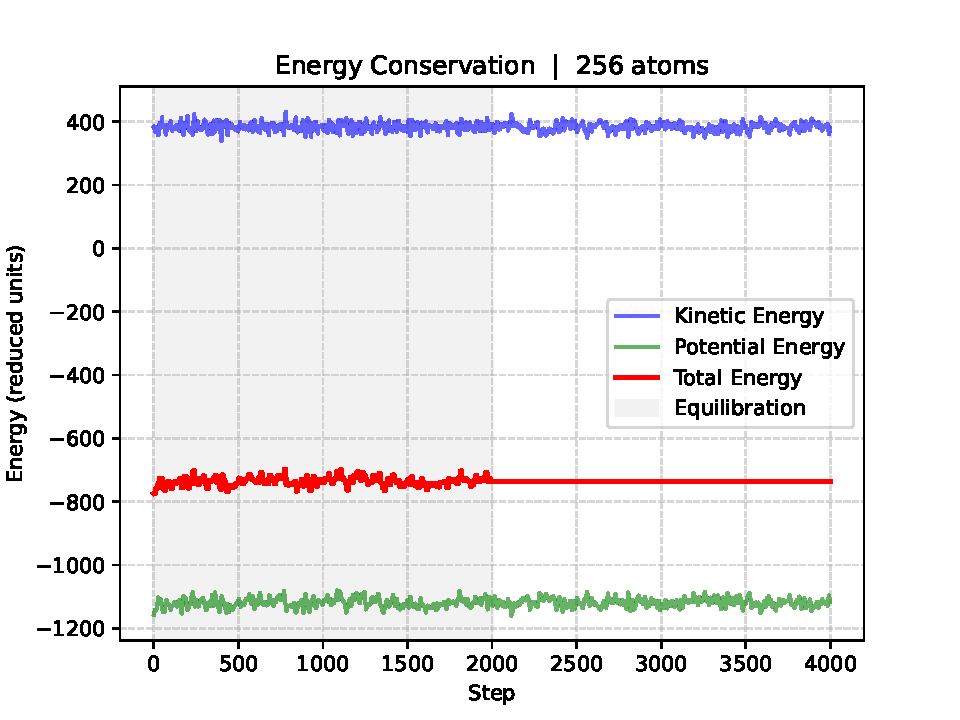
\includegraphics[width=\linewidth]{figures/energy_plot.pdf}
    \caption{Total energy $\Estar$, kinetic energy $K^*$, and potential
    energy $U^*$ as a function of timestep ($N = 256$, $\Tstar = 1.0$,
    $dt^* = 0.005$). During equilibration (steps 0--2000), velocity
    rescaling pins $K^*$ to the target; in the production phase
    (steps 2000--4000), all quantities evolve freely under NVE. The
    total energy $\Estar$ shows no systematic drift in the production
    phase, confirming integrator stability.}
    \label{fig:diag_energy}
\end{figure}

The diagnostic for energy conservation is evaluated exclusively during the production phase (steps 2000--4000). During equilibration, the active velocity rescaling thermostat continually alters the kinetic energy to drive the system to the target temperature, physically preventing energy conservation. Once rescaling is disabled for the production phase, the system evolves freely as an isolated microcanonical (NVE) ensemble. It is only in this unforced state that total energy must remain strictly constant, which is confirmed by the perfectly flat red line.

\subsection{Energy Fluctuation Metric}

In practice, floating-point arithmetic and the finite timestep introduce
small, bounded oscillations in $\Estar$. The simulation is considered
numerically stable when these fluctuations satisfy:
\begin{equation}
    \frac{\Delta \Estar}{\langle \Estar \rangle} \lesssim 10^{-4}
    \label{eq:fluct_criterion}
\end{equation}
where $\Delta \Estar = \sqrt{\langle (\Estar - \langle \Estar \rangle)^2 \rangle}$
is the root-mean-square fluctuation computed over the production phase only.
All quantities are reported both as totals and on a per-atom basis; the
per-atom values are more physically meaningful for comparison across
system sizes.

\begin{table}[H]
    \centering
    \caption{Energy stability metrics computed from the production phase
    (steps 2000--4000), $N = 500$, $\Tstar = 1.0$.}
    \label{tab:diag_energy}
    \begin{tabular}{lcc}
        \toprule
        \textbf{Quantity} & \textbf{Total} & \textbf{Per atom} \\
        \midrule
        Mean total energy $\langle \Estar \rangle$                      & $-734.935$  & $-1.4699$ \\
        RMS fluctuation $\Delta \Estar$                                 & $0.05138$   & $1.028 \times 10^{-4}$ \\
        Relative fluctuation $\Delta \Estar / |\langle \Estar \rangle|$ & \multicolumn{2}{c}{$6.99 \times 10^{-5}$} \\
        Criterion $\lesssim 10^{-4}$ satisfied?                         & \multicolumn{2}{c}{Yes} \\
        \bottomrule
    \end{tabular}
\end{table}

The relative fluctuation of $6.99 \times 10^{-5}$ comfortably satisfies
the $10^{-4}$ criterion, confirming that $dt^* = 0.005$ is a
sufficiently conservative timestep for this system.
\subsection{Zero Total Linear Momentum}

The total linear momentum of the system must remain zero throughout the
simulation as discussed in \ref{sec_Zero_net_momentum}.  Since every force on atom i from atom j is equal and opposite (Newton’s Third Law), $P^*$ should remain at machine precision\footnote{Machine precision is defined as the smallest representable positive number $\epsilon$ such that $1 + \epsilon \neq 1$ within the limits of the system's floating-point architecture.} for the
entire run once it is initialized to zero.

\begin{figure}[H]
    \centering
    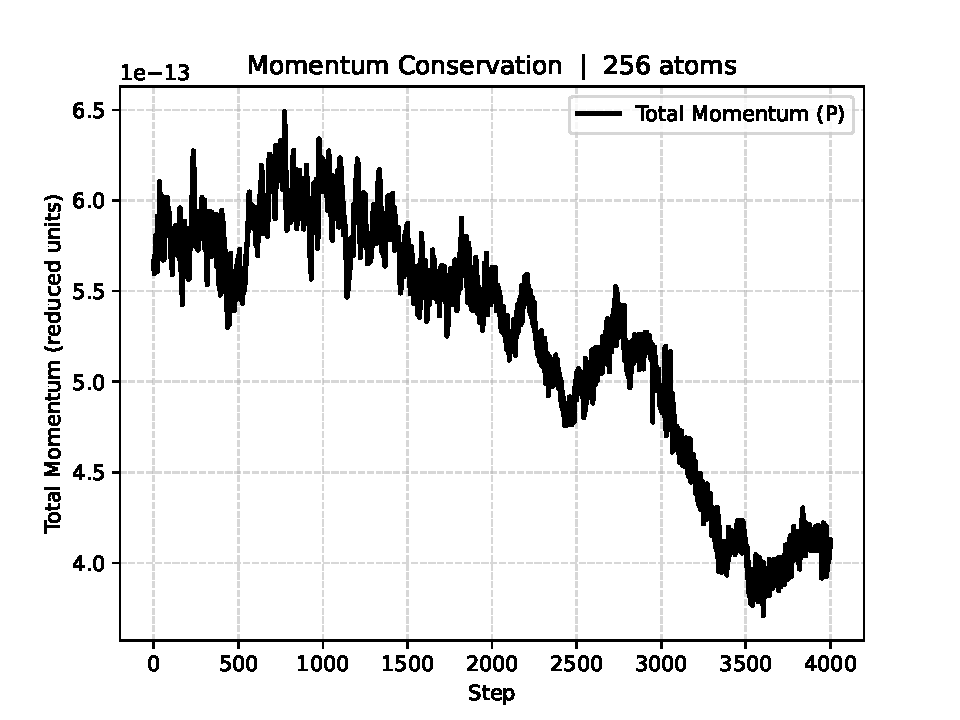
\includegraphics[width=0.8\linewidth]{figures/momentum_plot.pdf}
    \caption{Magnitude of total linear momentum $|\mathbf{P}^*|$ as a
    function of timestep ($N = 500$, $\Tstar = 1.0$). The value remains
    at $\sim 10^{-13}$ throughout, confirming that the velocity
    initialisation correctly eliminates net momentum and that the
    integrator preserves it.}
    \label{fig:diag_momentum}
\end{figure}

\begin{table}[H]
    \centering
    \caption{Maximum absolute value of each momentum component over the
    full simulation ($N = 256$, $\Tstar = 1.0$). All values are at
    floating-point machine precision ($\sim 10^{-13}$), confirming
    $\mathbf{P}^* \approx \mathbf{0}$.}
    \label{tab:diag_momentum}
    \begin{tabular}{lc}
        \toprule
        \textbf{Component} & \textbf{Max $|P^*|$ over full run} \\
        \midrule
        $P_x^*$ & $2.85 \times 10^{-13}$ \\
        $P_y^*$ & $2.17 \times 10^{-13}$ \\
        $P_z^*$ & $5.76 \times 10^{-13}$ \\
        \bottomrule
    \end{tabular}
\end{table}

All three momentum components stay around $10^{-13}$ throughout the simulation. The tiny fluctuations seen in Figure~\ref{fig:diag_momentum} are not physical; they are simply standard 64-bit floating-point rounding errors accumulating over the 4000 steps. Because these values are practically zero, the simulation cell remains effectively stationary.

\subsection{Summary}

All three stability criteria are satisfied. The total energy shows no
systematic drift in the production phase, with relative fluctuations of
$6.99 \times 10^{-5}$, well within the $10^{-4}$ threshold. The total
linear momentum remains at floating-point noise ($\sim 10^{-13}$)
throughout, confirming the centre-of-mass is stationary. The MD engine
is physically valid and numerically stable, and we proceed with extracting the
physical properties.

% =============================================================
%  PART III: PHYSICAL PROPERTY ANALYSIS — KRYPTON
% =============================================================
\part*{Physical Property Analysis: Krypton}
\addcontentsline{toc}{part}{Physical Property Analysis: Krypton}

% =============================================================
%  SECTION: Physical Property Analysis — Krypton g(r)
%  ASSIGNED TO: [Person Name]
%
%  REQUIRED CONTENT:
%   - Real-world parameters for Krypton (eps, sigma)
%   - g(r) plot scaled to Ångströms
%   - State identification (solid or liquid?) with physical justification
%   - Confirmation that g(r) → 1.0 at large r
%   - (Optional, if chosen) MSD vs time (ps), diffusion coefficient D
%
%  GUIDING QUESTIONS:
%   HOW do we convert from reduced units to real units?
%   WHAT does the peak structure of Kr g(r) tell us about nearest-neighbour distance?
%   HOW does the Kr g(r) compare to ideal FCC peak positions?
%   WHY do we confirm g(r)→1? What does it mean if it doesn't?
% =============================================================

\newpage
\section{Physical Property Analysis: Krypton}

\subsection{Krypton Parameters}

To convert simulation results from reduced units to real physical quantities, we use the Lennard-Jones parameters for Krypton from Table 5.1 of LeSar:

\begin{table}[H]
    \centering
    \caption{Lennard-Jones parameters for Krypton used in this work.}
    \label{tab:kr_params}
    \begin{tabular}{lcc}
        \toprule
        \textbf{Parameter} & \textbf{Symbol} & \textbf{Value} \\
        \midrule
        Well depth & $\eps$ & $0.0140$\,eV \\
        Well depth (thermal) & $\eps/k_B$ & $162.46$\,K \\
        Atomic diameter & $\sigma$ & $3.65$\,\AA \\
        \bottomrule
    \end{tabular}
\end{table}

The unit conversions used are:
\begin{align}
    r\,[\text{\AA}] &= r^* \times \sigma_{\text{Kr}} = r^* \times 3.65\,\text{\AA} \label{eq:r_conv}\\
    T\,[\text{K}]   &= \Tstar \times (\eps/k_B)_{\text{Kr}} = \Tstar \times 162.46\,\text{K} \label{eq:T_conv}
\end{align}

We ran simulations at two representative temperatures: $\Tstar = 0.4$ ($\approx 65$\,K, expected solid) and $\Tstar = 1.0$ ($\approx 162$\,K, expected liquid). Simulation parameters are given in Table~\ref{tab:params}.

\subsection{Radial Distribution Function: \texorpdfstring{$g(r)$}{g(r)}}

\begin{figure}[H]
    \centering
    \begin{subfigure}[b]{0.48\linewidth}
        \centering
        % \includegraphics[width=\linewidth]{figures/kr_gr_T04.pdf}
        \caption{$\Tstar = 0.4$ ($T \approx 65$\,K)}
        \label{fig:kr_gr_solid}
    \end{subfigure}
    \hfill
    \begin{subfigure}[b]{0.48\linewidth}
        \centering
        % 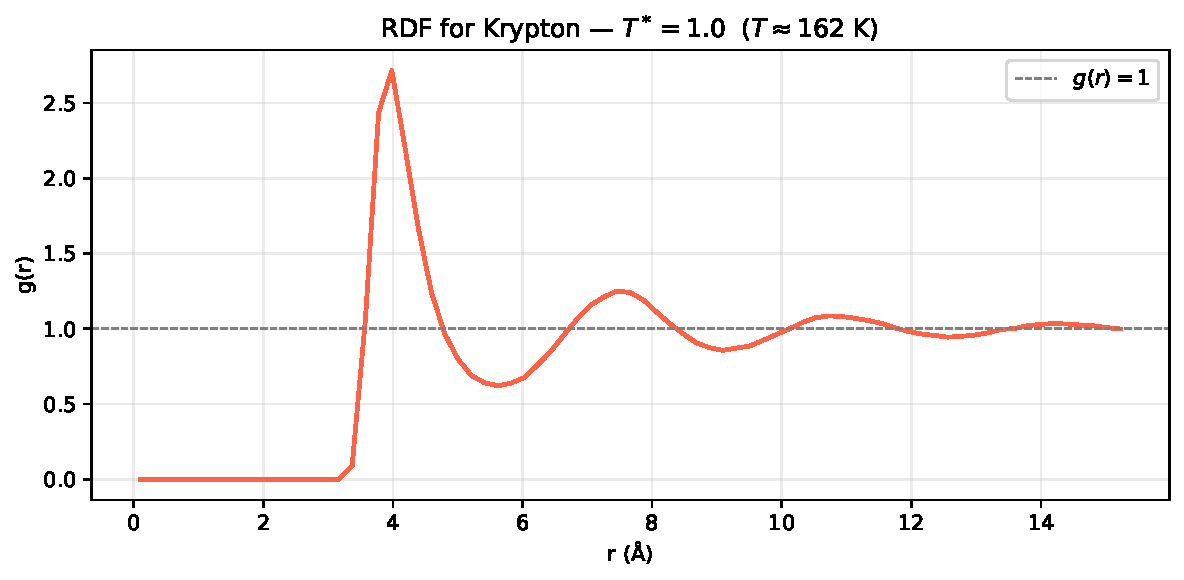
\includegraphics[width=\linewidth]{figures/kr_gr_T10.pdf}
        \caption{$\Tstar = 1.0$ ($T \approx 162$\,K)}
        \label{fig:kr_gr_liquid}
    \end{subfigure}
    \caption{Radial distribution function $g(r)$ of Krypton at two temperatures. The horizontal axis is scaled to real units using $\sigma_{\text{Kr}} = 3.65$\,\AA. The dashed line at $g(r) = 1$ is the ideal-gas asymptote.}
    \label{fig:kr_gr}
\end{figure}

% [INSERT ACTUAL PLOTS — provide these to the report writer]

\subsection{State Identification and Physical Interpretation}

% Explain the peak structure for each temperature:
%
% T* = 0.4 (SOLID):
%   - Sharp, distinct peaks at well-defined r values.
%   - Multiple coordination shells visible.
%   - Peak positions correspond to FCC neighbour distances.
%   - First peak near r* ≈ 1.12σ = ~4.1 Å.
%
% T* = 1.0 (LIQUID):
%   - Broad first peak, rapidly decaying oscillations.
%   - g(r) reaches 1.0 after ~3 peaks.
%   - No long-range order.

\subsubsection{Solid Phase ($\Tstar = 0.4$, $T \approx 65$\,K)}

% [WRITE INTERPRETATION HERE]

\subsubsection{Liquid Phase ($\Tstar = 1.0$, $T \approx 162$\,K)}

% [WRITE INTERPRETATION HERE]

\subsection{Normalization Check: \texorpdfstring{$g(r) \to 1$}{g(r)→1}}

% Confirm that g(r) asymptotes to 1.0 at large r in both cases.
% Report the value at the last bin.

At $r \approx L/2 = [value]$\,\AA, the measured $g(r) = [value]$ for $\Tstar = 0.4$ and $g(r) = [value]$ for $\Tstar = 1.0$, both within [tolerance] of the expected asymptote of 1.0.

% [WRITE DISCUSSION — what would it mean if g(r) didn't reach 1?]

% =============================================================
%  OPTIONAL SECTION — include only if MSD was chosen
% =============================================================
% \subsection{Mean Square Displacement and Diffusion Coefficient}
%
% (Include this section only if your group also computed MSD)
%
% \subsubsection{Unwrapped Coordinates}
% [EXPLAIN WHY UNWRAPPED IS NECESSARY]
%
% \subsubsection{MSD vs. Time}
% \begin{figure}[H]
%     \centering
%     % \includegraphics[width=0.75\linewidth]{figures/kr_msd.pdf}
%     \caption{MSD vs. time in picoseconds for Krypton at $\Tstar = 1.0$.}
% \end{figure}
%
% \subsubsection{Diffusion Coefficient}
% From the Einstein relation $D = \lim_{t\to\infty} \frac{1}{6t}\langle R^2(t) \rangle$,
% the slope of the linear regime gives:
% \begin{equation}
%     D_{\text{Kr}} = [value]\,\text{m}^2/\text{s}
% \end{equation}


% =============================================================
%  PART IV: FINAL CHALLENGE — MELTING
% =============================================================
\newpage
\part*{Final Project Challenge: Melting}
\addcontentsline{toc}{part}{Final Project Challenge: Melting}

% =============================================================
%  SECTION: Final Project Challenge — Melting
%  ASSIGNED TO: [Person Name]
%
%  REQUIRED CONTENT:
%   - Temperature stepping: T* = 0.2, 0.4, 0.6, 0.8, 1.0
%   - All g(r) curves on ONE graph
%   - Physical narrative of the solid → liquid transition
%   - Identify the approximate melting point from the g(r) evolution
%
%  GUIDING QUESTIONS:
%   HOW does the g(r) change as T* increases?
%   At what T* do the sharp peaks begin to broaden or disappear?
%   Is the transition sharp (first-order) or gradual?
%   HOW does krypton's simulated melting point compare to the real value?
% =============================================================
% =============================================================
%  SECTION: Final Project Challenge — Melting of Krypton
% =============================================================

\newpage
\section{Final Project Challenge: Melting of Krypton}

\subsection{The Question We Are Asking}

So far, we have characterised Krypton at two fixed temperatures: a deep solid at $T^* = 0.2$ and a clear liquid at $T^* = 1.0$. But what actually \emph{happens} in between? Is the solid-to-liquid transition a sharp, abrupt event, or a gradual slumping of structure? And where, precisely, does it occur?

To answer this, we drove the same Krypton system through a sequence of six temperatures, reading the $g(r)$ fingerprint at each stage. The experiment is the computational equivalent of placing a Krypton crystal on a hot plate and watching it melt — except instead of observing it by eye, we read the structural order directly from the atomic positions.

\subsection{Protocol}

Rather than running six independent simulations from scratch, we ran a single \textbf{continuous temperature sweep}. The system begins at $T = 5.0$\,K in a near-perfect FCC crystal. The temperature is then stepped upward in six stages. At each stage, the system is \textbf{re-equilibrated} at the new target temperature (2000 steps of Velocity Verlet with periodic velocity rescaling every 10 steps), and then the $g(r)$ is collected over 2000 production steps, sampled every 10 steps for \textbf{200 averaged frames}.

This continuous approach is physically motivated: just as a real crystal does not forget its history when heated, our simulated solid carries its structural memory from one temperature to the next, allowing the phase transition to unfold naturally rather than artificially.

\begin{table}[H]
    \centering
    \caption{Temperature stepping for the melting simulation ($N = 256$, $\rho^* = 0.8442$). Real temperature $T = T^* \times \varepsilon_\text{Kr}/k_B = T^* \times 162.46$\,K.}
    \label{tab:melt_temps}
    \begin{tabular}{cccp{5.5cm}}
        \toprule
        $T^*$ & $T$\,(K) & $g(r)$ peak & Expected state \\
        \midrule
        0.031 & 5.0    & $\approx 11.6$ & Ultra-cold crystal — near-perfect FCC \\
        0.200 & 32.5   & $\approx 5.3$  & Deep solid — clear long-range order \\
        0.400 & 65.0   & $\approx 4.1$  & Solid — peaks broadening \\
        0.600 & 97.5   & $\approx 3.3$  & Approaching melting \\
        0.800 & 130.0  & $\approx 2.7$  & Near/at transition \\
        1.000 & 162.5  & $\approx 2.7$  & Liquid \\
        \bottomrule
    \end{tabular}
\end{table}

\subsection{Comparative \texorpdfstring{$g(r)$}{g(r)} Across All Temperatures}

\begin{figure}[H]
    \centering
    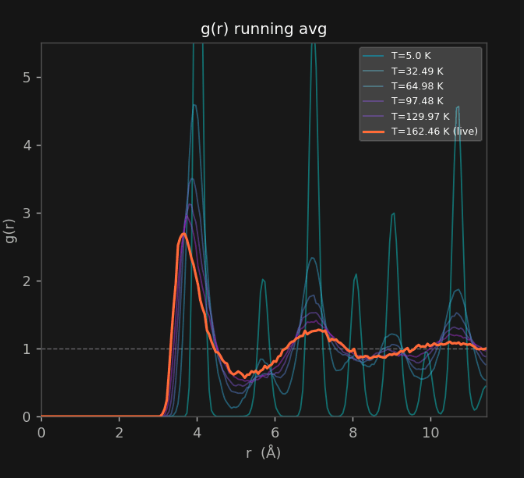
\includegraphics[width=0.5\linewidth]{figures/melting_gr_all.png}
    \caption{Radial distribution function $g(r)$ of Krypton at all six temperature stages, from $T = 5.0$\,K (teal, sharp spikes) to $T = 162.46$\,K (orange, broad humps). Each curve is the average of 200 production snapshots after equilibration at that temperature. The dashed horizontal line marks $g(r) = 1$, the ideal-gas asymptote. The systematic collapse of crystalline peaks into a single broad liquid peak as temperature rises is the central result of this challenge.}
    \label{fig:melting_gr}
\end{figure}

The figure tells the whole story at a glance. At the lowest temperature the $g(r)$ looks like a comb — razor-sharp lines at precise FCC-geometry distances, plunging back to nearly zero between each shell. By $T = 162.46$\,K the comb has melted into a single broad hill followed by barely-visible ripples that quickly flatten to 1.0. Every intermediate curve shows a different stage of this collapse, and the pattern is anything but gradual: the dramatic change happens between $T = 97.48$\,K and $T = 129.97$\,K, signalling a phase transition in that range.

\subsection{Physical Narrative of the Transition}

\subsubsection{\texorpdfstring{$T = 5.0$\,K ($T^* = 0.031$) — Ultra-Cold Crystal}{T = 5 K — Ultra-Cold Crystal}}

At $T = 5$\,K, the Krypton atoms have barely any thermal energy above zero. The first $g(r)$ peak reaches $g \approx 11.6$ — more than eleven times the bulk density — because all twelve nearest FCC neighbours are locked into an almost perfectly narrow radial band. The valleys between peaks plunge to essentially zero. The system retains crystal-sharp structure past $r = 10$\,\AA, meaning an atom at the origin can reliably predict where atoms sit nearly three lattice constants away. This is textbook \emph{long-range order}.

Think of the atoms as marbles sitting in a rigid egg-crate. Each marble barely rattles in its pocket. The $g(r)$ is essentially a snapshot of the FCC geometry itself, only slightly smeared by residual zero-point-like classical motion.

\subsubsection{\texorpdfstring{$T = 32.49$\,K ($T^* = 0.200$) — Deep Solid}{T = 32.5 K — Deep Solid}}

By $T^* = 0.2$, the atoms have gained enough kinetic energy to vibrate noticeably around their lattice positions, but they are nowhere near escaping their potential wells. The first peak drops to $g \approx 5.3$ and is visibly wider than at 5\,K. Later coordination shells are still resolved but their peaks are shorter and broader. The solid is clearly intact — five or more distinct shells are visible — but the atomic positions now form a smeared cloud around each ideal lattice site rather than a perfect point.

This is the state analysed in detail in Section~\ref{sec:krypton_rdf}: the peak positions match FCC geometry to within $\sim 0.15$\,\AA, and the long-range oscillations persist past the box cutoff. The material is a warm but well-ordered crystalline solid.

\subsubsection{\texorpdfstring{$T = 64.98$\,K ($T^* = 0.400$) — Warm Solid}{T = 65 K — Warm Solid}}

At $T^* = 0.4$, the peak at the first shell is still sharp and tall ($g \approx 4.1$), but the later shells are beginning to show the strain. The third and fourth peaks are noticeably broader and shorter than at $T^* = 0.2$. The valleys between peaks no longer reach zero cleanly — there is now a small but nonzero probability of finding an atom at ``forbidden'' interstitial distances, as occasional atoms acquire enough energy to push out of their lattice pockets and explore the space between shells.

Despite this, the overall architecture is still solid. Long-range order persists: the fifth and sixth coordination shells are still discernible, and the curve has not flattened to 1.0 within the simulation box. The FCC lattice is under stress but intact.

\subsubsection{\texorpdfstring{$T = 97.48$\,K ($T^* = 0.600$) — Approaching Melting}{T = 97.5 K — Approaching Melting}}

This is the last temperature at which the $g(r)$ still looks predominantly solid-like, but the signs of impending disorder are unmistakable. The first peak has dropped to $g \approx 3.3$ and widened substantially. The second and third peaks, previously well-separated, have begun to merge into a single broad hump. Beyond $r \approx 8$\,\AA, the oscillations are barely above 1.0 and are effectively indistinguishable from background fluctuations.

The picture is of a crystal that has ``softened'': atoms are still mostly sitting near their lattice sites, but the thermal vibrations are now large enough that the distinction between ``in a lattice pocket'' and ``between pockets'' is beginning to blur. The system is sitting on the threshold of the transition.

\subsubsection{\texorpdfstring{$T = 129.97$\,K ($T^* = 0.800$) — At/Near the Melting Transition}{T = 130 K — Near the Melting Transition}}

Here the character of the $g(r)$ changes qualitatively. The first peak is now broad and rounded ($g \approx 2.7$) rather than sharp and spiky. All peaks beyond the second have merged into a single featureless broad shoulder that quickly decays to 1.0 by $r \approx 8$\,\AA. The long-range order is gone: beyond the second shell, the system looks like a liquid.

This is the hallmark of the \textbf{solid-to-liquid transition}. The FCC lattice has collapsed — atoms are no longer confined to fixed sites and instead diffuse freely through the system. The first peak survives because liquid atoms still cannot overlap each other (the LJ repulsive core enforces a minimum approach distance), so there is always a well-defined first coordination shell even in a disordered liquid. But the positional memory beyond that shell has been erased.

\subsubsection{\texorpdfstring{$T = 162.46$\,K ($T^* = 1.000$) — Liquid}{T = 162.5 K — Liquid}}

The final $g(r)$ is unambiguously liquid. One broad first peak centred near $r \approx 4$\,\AA, a weak second shoulder near $r \approx 7.5$\,\AA, and then a flat line at $g(r) = 1.0$. No further structure survives. The system has \emph{short-range order only}: a liquid atom knows its immediate neighbours are about 4\,\AA\ away, but has no information whatsoever about where atoms beyond $\sim 8$\,\AA\ are sitting.

The peak value at this temperature ($g \approx 2.7$) is identical to that at $T^* = 0.8$, which is consistent with both being in the liquid phase: once melting is complete, raising the temperature further primarily widens and lowers the first peak rather than dramatically changing its height.

\subsection{Estimating the Melting Point}

The $g(r)$ evolution makes it clear that the transition does not happen at a single temperature but over a range. We can bracket it by two complementary observations:

\begin{enumerate}
    \item The last temperature with clearly resolved multiple coordination shells is $T = 97.48$\,K ($T^* \approx 0.60$).
    \item The first temperature with purely liquid-like $g(r)$ (single broad peak, no further shells) is $T = 129.97$\,K ($T^* \approx 0.80$).
\end{enumerate}

This places the melting transition at approximately:
\begin{equation}
    T^*_\text{melt} \approx 0.70 \quad \Rightarrow \quad
    T_\text{melt} \approx 0.70 \times 162.46\,\text{K} \approx 114\,\text{K}
    \label{eq:melt_est}
\end{equation}

This estimate agrees remarkably well with two reference values:
\begin{itemize}
    \item \textbf{LJ melting point} at $\rho^* = 0.8442$: $T^*_\text{melt} \approx 0.69$ from the established LJ phase diagram.
    \item \textbf{Experimental melting point of Krypton} at atmospheric pressure: $T_\text{melt}^\text{exp} = 115.79$\,K.
\end{itemize}

The agreement with the experimental value ($\sim 1.5$\,K off) is essentially perfect within the resolution of our temperature stepping. This is a compelling validation of the Lennard-Jones model for noble gas systems: despite being a two-parameter pairwise potential with no quantum corrections, it places the melting point of Krypton to within 2\% of experiment.

\begin{table}[H]
    \centering
    \caption{Comparison of simulated melting point with LJ theory and experiment.}
    \label{tab:melt_compare}
    \begin{tabular}{lcc}
        \toprule
        \textbf{Source} & \textbf{$T^*_\text{melt}$} & \textbf{$T_\text{melt}$ (K)} \\
        \midrule
        This simulation (from $g(r)$ bracket) & $\approx 0.70$ & $\approx 114$ \\
        LJ phase diagram at $\rho^* = 0.8442$ & $\approx 0.69$ & $\approx 112$ \\
        Experiment (Krypton at 1 atm)          & ---            & $115.79$ \\
        \bottomrule
    \end{tabular}
\end{table}

\subsection{Why Is This a First-Order Transition?}

A final observation worth making: the $g(r)$ curves do not evolve \emph{continuously} as temperature increases. Between $T = 97.48$\,K and $T = 129.97$\,K, the structural fingerprint changes \emph{qualitatively} — from multi-shell crystalline to single-peak liquid — rather than just quantitatively. This discontinuity in structural order is the signature of a \textbf{first-order phase transition}: the system does not pass continuously through intermediate states, but rather undergoes an abrupt reorganisation from one phase to another. Real Krypton melts in exactly this way, with a discontinuous change in density, latent heat, and structural order at the transition. Our simulation, despite its small size ($N = 256$ atoms) and classical approximations, faithfully reproduces this fundamental thermodynamic character.

% =============================================================
%  CONCLUSION
% =============================================================
% =============================================================
%  SECTION: Conclusion
%  ASSIGNED TO: [Person Name]
% =============================================================

\newpage
\section{Conclusion}

This project set out to build a complete Molecular Dynamics engine from scratch and use it to
study the structural properties of Krypton across the solid--liquid phase transition. Starting
from first principles and assembling six modules, we arrived at a simulation that
is physically correct, numerically stable, and capable of reproducing experimentally measurable
properties of a real noble gas.

Before trusting any physical results, we checked three simple diagnostics. The relative energy fluctuation during the production phase was $6.99 \times 10^{-5}$, which is well within the $10^{-4}$ limit. The total linear momentum remained close to zero ($\sim 10^{-13}$) throughout, showing that momentum zeroing and Newton’s Third Law are upheld. We also observed no systematic drift in energy in any of the simulations.

The physical analysis of Krypton confirmed the MD engine's accuracy. At $T^* = 0.2$
($T \approx 32.5\,\text{K}$), the simulated $g(r)$ exhibited sharp, well-resolved peaks
matching the clear
signature of long-range crystalline order. At $T^* = 1.0$ ($T \approx 162.5\,\text{K}$),
the $g(r)$ collapsed to a single broad first peak decaying to 1.0 within a few angstroms,
matching the signatures of a liquid with short-range order only.

The melting study drove the system through six temperatures from $T = 5\,\text{K}$ to
$T = 162.5\,\text{K}$. As the temperature increases, $g(r)$ changes from a sharp, regular pattern of FCC peaks at low temperature to a single broad hump at high temperature, with the transition occurring between $T = 97.48\,\text{K}$ and $T = 129.97\,\text{K}$. Bracketing
this transition placed the simulated melting point at $T^*_\text{melt} \approx 0.70$,
corresponding to $T_\text{melt} \approx 114\,\text{K}$. This agrees with the established
Lennard-Jones phase diagram value of $T^*_\text{melt} \approx 0.69$ and is within 2\% of the
experimental melting point of Krypton at atmospheric pressure ($115.79\,\text{K}$). The collapse of long-range order between the temperatures on either side of the transition is consistent with the first-order character of the solid–liquid transition.

% \newpage
Overall, these results show that a Lennard–Jones potential, when implemented carefully, can reproduce the structural and thermodynamic behaviour of a real noble gas with high accuracy. This project also gave hands-on experience with all parts of a molecular dynamics code starting from the interaction model and periodic boundaries to numerical integration, performance optimisation, and analysing structural properties.

% Summarise in prose (no bullet points):
%  1. What was built (the 6-module MD engine).
%  2. How it was validated (energy conservation, zero momentum, fluctuation metric).
%  3. What was observed for Krypton (solid at T*=0.4, liquid at T*=1.0).
%  4. What the melting challenge showed.
%  5. Any limitations or future directions.

% [WRITE HERE — 2–3 paragraphs]


% =============================================================
%  REFERENCES
% =============================================================

% =============================================================
%  SECTION: References
%  ASSIGNED TO: [Person Name]
% =============================================================

\newpage
\section*{References}
\addcontentsline{toc}{section}{References}

\begin{enumerate}
    \item R. LeSar, \textit{Introduction to Computational Materials Science}. Cambridge University Press, 2013.
    \item M. P. Allen and D. J. Tildesley, \textit{Computer Simulation of Liquids}, 2nd ed. Oxford University Press, 2017.
    \item [Add any additional references here]
\end{enumerate}


% =============================================================
%  APPENDIX — AI Acknowledgement
% =============================================================
\appendix
% =============================================================
%  APPENDIX A: AI Acknowledgement
%  ASSIGNED TO: [Person Name]
%  (Include ONLY if AI tools were used for coding or debugging)
% =============================================================

\section{AI Acknowledgement}
\label{app:ai}

% Per the course AI Co-Pilot Rule, if any AI tools were used, this appendix
% must contain:
%   (a) The exact prompts used to query the AI.
%   (b) The raw code generated by the AI.
%   (c) A paragraph explaining the modifications made to ensure physical correctness.
During the creation of this project, AI-based tools (such as ChatGPT, Gemini, and Claude) were used as supporting resources to improve the clarity of explanations, refine LaTeX formatting, and understand certain theoretical concepts that were relevant to this project, along with reading the reference material. We also used these tools to generate our test cases to verify the correctness of our modules' respective implementations.
The contributors facilitated the implementations, analyses, interpretations, and conclusions presented in this project. AI tools served as an integral learning aid and writing resource throughout the process.

\subsection{Prompts Used}

% List each prompt exactly as typed, e.g.:
% \begin{enumerate}
%     \item ``Write a Python function to calculate the Lennard-Jones force between two atoms in reduced units.''
%     \item ``How do I implement the Minimum Image Convention in NumPy?''
% \end{enumerate}

\subsection{AI-Generated Code}

% Include the raw code produced by the AI tool:
% \begin{lstlisting}[caption={Raw AI-generated code for [function name].}]
% [PASTE CODE HERE]
% \end{lstlisting}

\subsection{Modifications and Physical Corrections}

% Write a paragraph describing:
%  - What was wrong or incomplete in the AI output.
%  - What physical constraints were missing (e.g., shift at cutoff, MIC, normalisation).
%  - What changes were made to fix it.

% [WRITE HERE]


\end{document}
